\definecolor{Gray2}{rgb}{ .851,  .851,  .851}
\chapter{Vuelo Horizontal}

Las condiciones para el vuelo rectilíneo son sencillas: la velocidad vertical ha de ser nula, mientras que la horizontal no. Con estas condiciones y a nivel del mar se pueden obtener las gráficas \ref{PMVH}, \ref{ControlVH}, \ref{EulerVH} y \ref{PVH}, que ofrecen una primera aproximación del rendimiento de la aeronave en configuración sin carga de pago. De ellas se puede deducir que el valor de potencia total mínimo es de 27,307 kW, y se da para una velocidad de vuelo de 28.73 m/s. Para calcular la velocidad máxima de avance es necesario obtener características del motor, el cual no se ha decidido, por lo que, para tener unos valores orientativos, se ha optado por emplear los datos del motor que monta el Cicaré 7B, un helicóptero de peso similar al vehículo a diseñar. El motor en cuestión es el ROTAX 912 ULS, un motor de 4 tiempos y 4 cilindros, con un consumo especifico de 285 g/kW$\cdot$ h a una potencia máxima continua de 58 kW a 5500 rpm \citep{ROTAX}. Con esta limitación reflejada en la gráfica \ref{PMVH} se puede observar que el motor, cuya potencia máxima continua disponible es de 58 kW, permite volar a velocidades de hasta 68.28 m/s en estas condiciones.

\begin{figure}
	\centering
	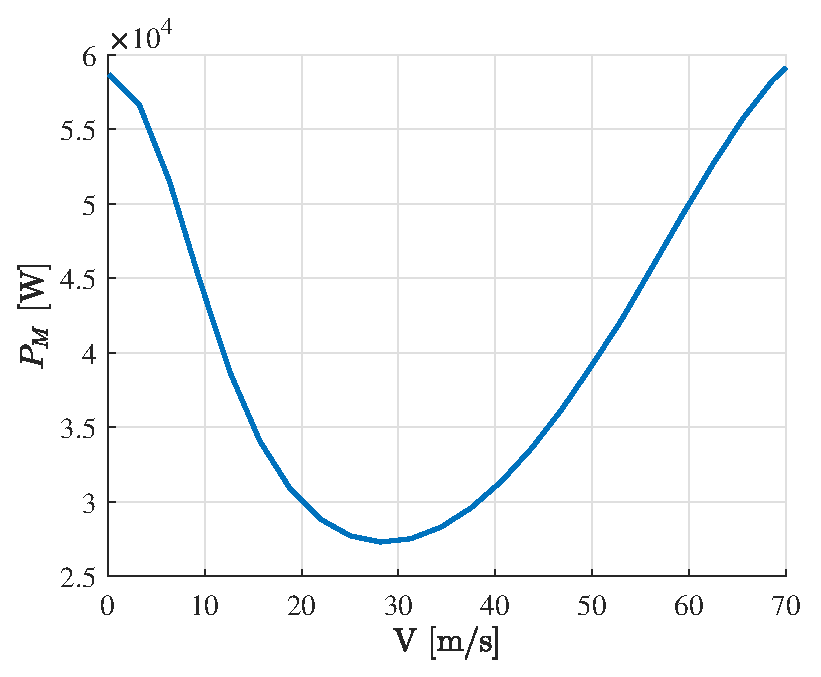
\includegraphics[width=90mm]{graficos/PMVH}
	\caption{Consumo de Potencia de la aeronave en función de la velocidad de vuelo a nivel del mar para vuelo horizontal y limitación por potencia máxima continua disponible.}
	\label{PMVH}
\end{figure}
\begin{figure}
	\centering
	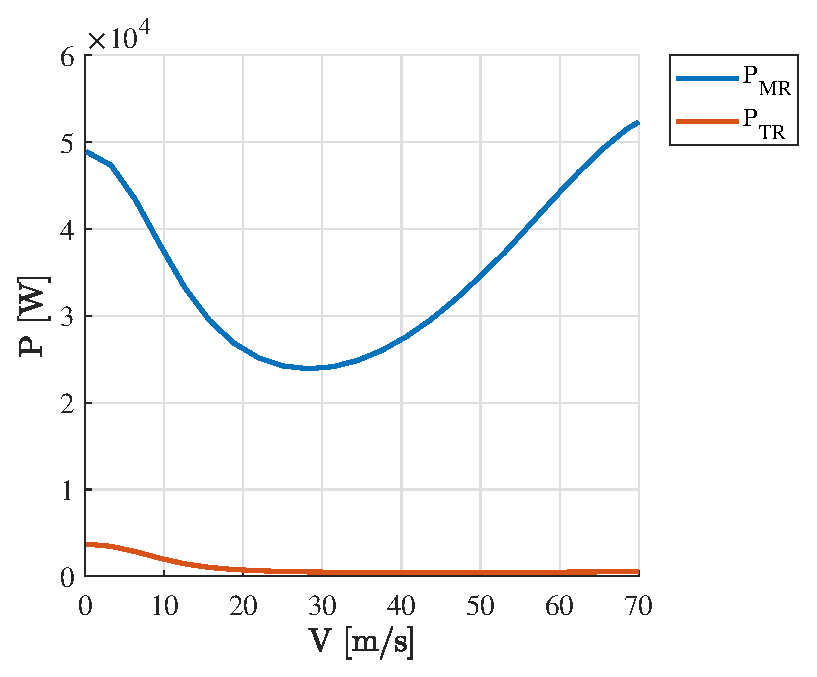
\includegraphics[width=90mm]{graficos/PVH}
	\caption{Consumo de Potencia de los rotores principal y antipar en función de la velocidad de vuelo a nivel del mar para vuelo horizontal.}
	\label{PVH}
\end{figure}
\begin{figure}
	\centering
	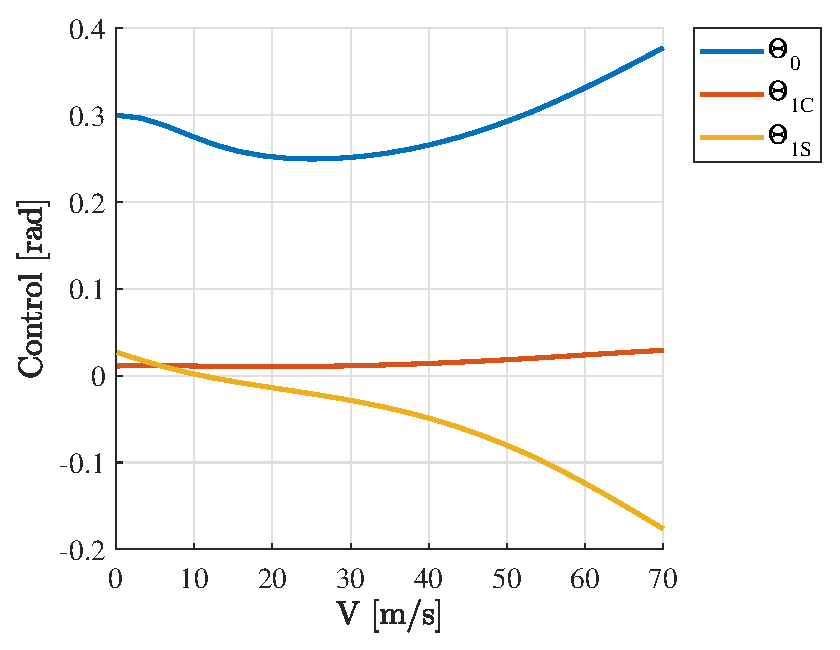
\includegraphics[width=90mm]{graficos/ControlVH}
	\caption{Ángulos de control de la aeronave en función de la velocidad de vuelo a nivel del mar para vuelo horizontal.}
	\label{ControlVH}
\end{figure}
\begin{figure}
	\centering
	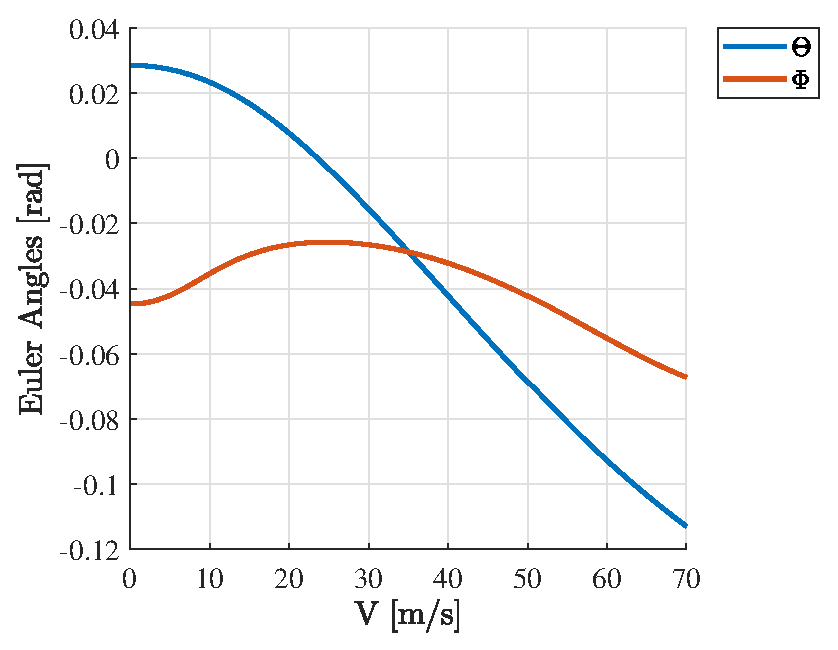
\includegraphics[width=90mm]{graficos/EulerVH}
	\caption{Ángulos de Euler de la aeronave en función de la velocidad de vuelo a nivel del mar para vuelo horizontal.}
	\label{EulerVH}
\end{figure}

\section{Autonomía de Vuelo}

Con estos datos se puede hacer una estimación de la autonomía del vehículo. 
Para poder obtener el consumo específico del motor en las condiciones de vuelo de máxima autonomía, se emplea el modelo recogido en \citet{Cuerva}, que calcula el consumo en función de la potencia necesaria para el vuelo.
\begin{equation}
	c_e(P)=\frac{c_{e,P_{max}}}{1+\frac{K_m}{c_{e,P_{max}}}(1-\frac{P_{max}}{P(t)})}
	\label{consumo}
\end{equation}
Donde $c_e$ es el consumo específico al régimen de vuelo considerado, $c_{e,P_{max}}$ el consumo específico del motor en régimen de funcionamiento de máxima potencia, $P_{max}$ la potencia máxima continua capaz de ofrecer el motor y $P$ la potencia necesaria para el vuelo considerado.
$K_m$ es un parámetro que mide la eficiencia del motor, que en motores muy eficientes es del orden de 8.33$\cdot$10$^-9$ kg/W$\cdot$s (0.03 kg/kW$\cdot$h).
Además se suponen unas cargas de combustible del 9\% del MTOW del vehículo. 

Lo siguiente es decidir un modelo de cálculo de la autonomía, ya que no se dispone de datos suficientes para hacer unos cálculos exactos,ni estos son necesarios en una fase de diseño preliminar. La hipótesis básica es considerar las masa del vehículo constante durante el vuelo, cosa que no es así por el consumo del propio combustible, pero simplificará los cálculos en gran medida.
Para los cálculos se empleará el método del equilibrado del helicóptero, que permite incluir gran cantidad de información en los cálculos y por tanto aumentar la fiabilidad de estos. Como se desarrollará a continuación, la complejidad de este método reside en el propio equilibrado del helicóptero, que permitirá obtener el valor de potencia requerido para el vuelo, a partir del cual el cálculo de la autonomía resulta trivial.

En \citet{Filippone} se expone un método para calcular la autonomía de forma sencilla empleando para ello la potencia (calculada mediante el equilibrado) del vuelo y el consumo específico (calculado mediante la ecuación \ref{autonomia}).
Se define la autonomía específica $E_s$
\begin{equation}
	E_s=\frac{\partial t}{\partial m}=\frac{1}{\dot{m_f}}=\frac{1}{P\cdot c_{e}(P)}
	\label{autespecifica}
\end{equation}
y con la hipótesis de masa constante solo es necesario resolver el equilibrado para una velocidad ya que
\begin{equation}
	\frac{\partial P}{\partial t}=0\rightarrow P=cte
\end{equation}
que al introducir en la ecuación \ref{consumo} se obtiene que
\begin{equation}
	P=cte\rightarrow c_e=cte
\end{equation}
y por tanto
\begin{equation}
E_s=\frac{1}{P\cdot c_{e}}=cte
\label{autespecificacte}
\end{equation}
Una vez obtenido el valor de la autonomía especifica, el calculo de la autonomía resulta sencillo
\begin{equation}
	t_{e}=E_s\cdot \Delta m=E_s\cdot MFM=\frac{MFM}{c_e\cdot P}
	\label{autonomia}
\end{equation}

Donde $t_e$ es la autonomía, $MFM$ es la masa máxima de combustible, $C_{e}$ es el consumo específico y $P_e$ la potencia en el régimen de de vuelo.
La tabla \ref{auttabla} recoge los datos necesarios para el cálculo de la autonomía máxima y el valor de esta.

\begin{table}[htbp]
	\centering
	\begin{tabular}{|>{\columncolor{Gray}}c|c|}
		\hline
		\cellcolor{Gray2}Variable & \cellcolor{Gray2}Valor \\ \hline \hline
		\cellcolor{Gray}Potencia para máxima autonomía ($P_{min,t_{e,max}}$)  & 27.307 kW \\ \hline
		\cellcolor{Gray}Velocidad en régimen de máxima autonomía ($V$) & 28.73 m/s \\ \hline
		\cellcolor{Gray}Consumo específico en régimen de máxima autonomía ($c_{e,t_{e,max}}$) & 8.98$\cdot$10$^-08$ kg/W$\cdot$s \\ \hline
		\cellcolor{Gray}Máxima autonomía ($t_{e,max}$) & 4.5887 h \\ \hline
	\end{tabular}%
	\caption{Parámetros relativos al cálculo de la máxima autonomía y su valor para un vuelo horizontal a nivel del mar.}
	\label{auttabla}
\end{table}%

A modo de comprobación, se han calculado las autonomías correspondientes a distintas velocidades de vuelo en la gráfica \ref{teVH}. Se puede observar que su forma resulta muy similar a la de la gráfica \ref{PMVH} pero invirtiéndola según el eje x. Esto se debe a que la autonomía no depende de otro parámetro de vuelo que no sea la potencia consumida, por lo que la evolución de la potencia necesaria será inversa a la evolución de la autonomía de vuelo, siendo el mínimo de potencia necesaria el máximo de autonomía.

\begin{figure}
	\centering
	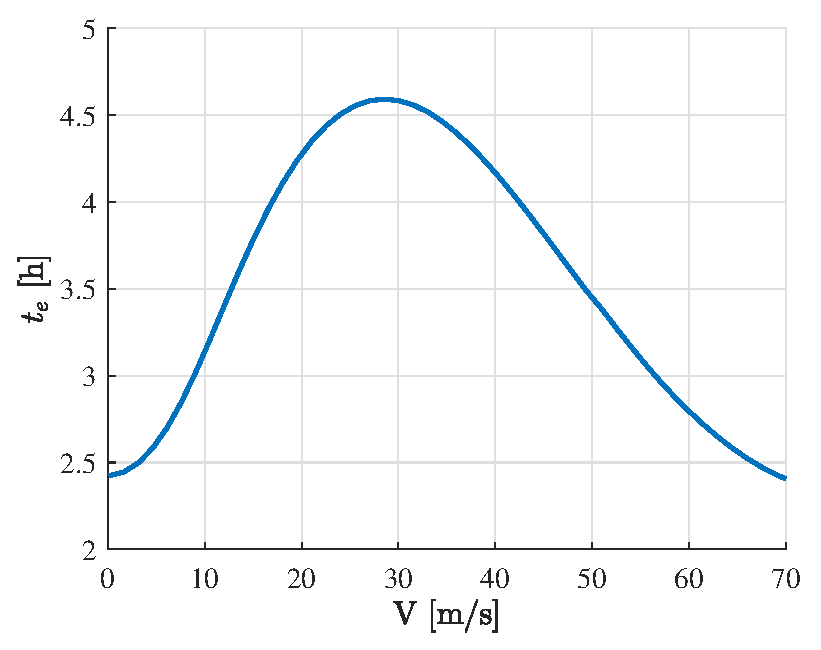
\includegraphics[width=90mm]{graficos/teVH}
	\caption{Autonomía de la aeronave en función de la velocidad de vuelo a nivel del mar para vuelo horizontal.}
	\label{teVH}
\end{figure}
%Los datos del motor son
%Pot. Max. Coontinua 58 Kw
%consumo l/h 22,6 (100%) y 16,2 (75%)
%consumo especifico al 100% 285g/kWh
%Con el la potencia de máxima autonomía a 31,5kW, una regla de 3 nos dice que el consumo es un 51.9069026% del de maxima potencia,regla de 3, no 100% seguro.

%\section{Fuerzas y Momentos Sobre los Elementos de la Cola}
%
%En futuras fases de diseño será necesario definir el diseño estructural y los materiales con los que se construirá la aeronave, por lo que puede ser interesante realizar un análisis de las fuerzas que deberán soportar algunos elementos para tener una idea aproximada de las cargas que pueden aparecer en servicio.
%
%De entre estas cargas, las que aparecen en los elementos de la cola son muy importantes, ya que los momentos flectores inducidos por estas cargas en la propia cola pueden ser grandes debido a la longitud de esta, y habrá que diseñarla de tal manera que las posibles deformaciones que aparezcan en funcionamiento no interfieran en el mismo.
%
%Las figuras \ref{FAP} y \ref{FE} representan los valores de las fuerzas que aparecen en el rotor antipar y estabilizadores vertical y horizontal para cada velocidad de vuelo considerada. Solo se representas las cargas que tienen algún valor de interés, por ejemplo, las cargas en el eje y que se den en el estabilizador horizontal serán despreciables y no serán relevantes a la hora de calcular las cargas sobre la cola.
%
%\begin{figure}
%	\centering
%	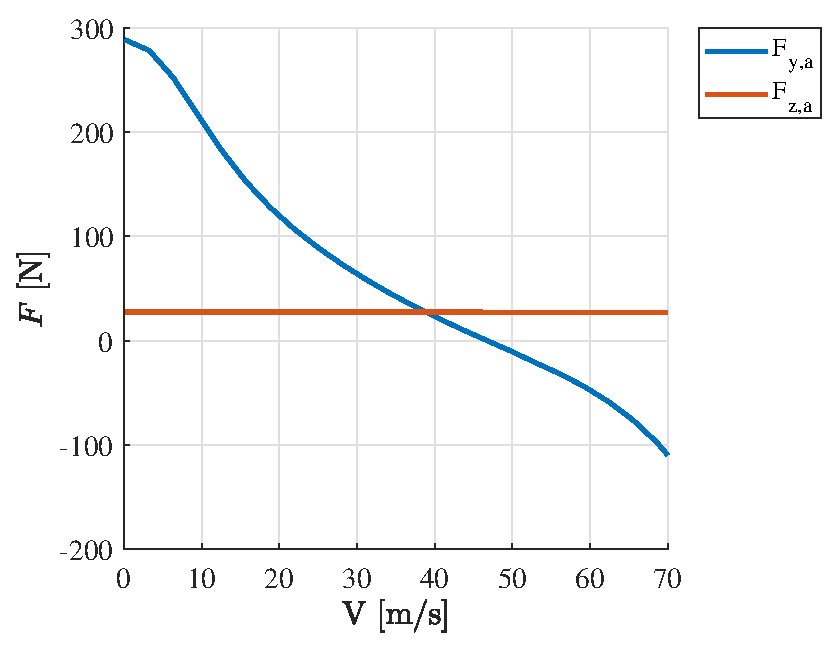
\includegraphics[width=90mm]{graficos/FAP}
%	\caption{Fuerzas sobre el rotor antipar a distintas velocidades de vuelo a nivel del mar según los ejes cuerpo y y z.}
%	\label{FAP}
%\end{figure}
%
%\begin{figure}
%	\centering
%	\subfigure[Estabilizador vertical]{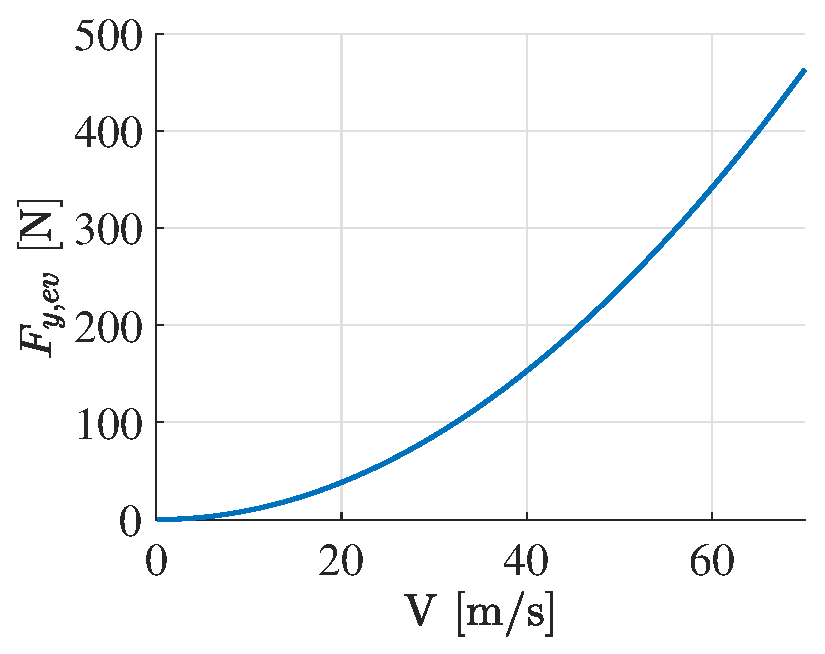
\includegraphics[width=60mm]{graficos/FEV}}
%	\subfigure[Estabilizador horizontal]{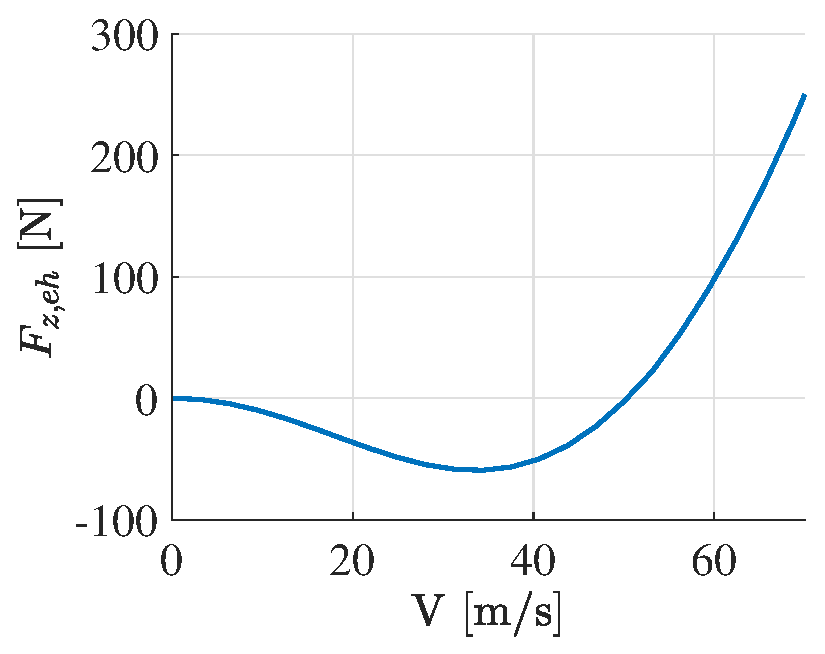
\includegraphics[width=60mm]{graficos/FEH}}
%	\caption{Fuerzas sobre los estabilizadores (a) vertical y (b) horizontal a distintas velocidades de vuelo a nivel del mar. Las fuerzas que se representan son horizontales (eje y cuerpo) para el estabilizador vertical y verticales (eje z cuerpo) para el estabilizador vertical.}
%	\label{FE}
%\end{figure}
%
%
%Se puede observar en la gráfica \ref{FAP} que las cargas sobre el rotor antipar cambian de signo, es decir, de sentido, a partir de ciertas velocidades. Esta evolución puede resultar extraña, pero el motivo se puede observar en la gráfica \ref{FAP}. Como ocurriría con un ala, el estabilizador vertical genera una carga en el eje y que aumenta con la velocidad de vuelo. Esta carga ayuda a reducir la potencia necesaria en el rotor antipar para bajas velocidades ya que ayuda a compensar el momento de giro que provoca el rotor principal. Sin embargo, estas cargas, para velocidades altas, superan a las necesarias para compensar dicho momento, y el antipar debe pasar a compensar la carga sobre el estabilizador vertical. Además, aunque su origen no es aerodinámico, el propio peso del rotor antipar supondrá una carga de valor constante que también se ha de tener en cuenta.
%
%En lo que respecta al estabilizador horizontal, a bajas velocidades genera una carga ascendente que ayuda a la estabilidad longitudinal del sistema. A altas velocidades (mayores a 50 m/s) las cargas se vuelven descendentes. Esto puede deberse a un fallo del modelo, que en situaciones límite no sea capaz de obtener buenas aproximaciones, aunque en una situación real en avance, la estela del rotor principal puede incidir sobre el estabilizador horizontal y generar cargas descendentes.
%
%Queda por tanto claro que a mayor velocidad de vuelo las cargas serán mayores, llegando hasta cargas de 300 N que la cola tendrá que soportar en vuelo a punto fijo (debidas al rotor antipar), pero mayores para vuelos a altas velocidades (400 N para vuelos a 60 m/s).
%
%\subsection{Variación de las Cargas en la Cola con el Ángulo de Ataque $\boldsymbol{\alpha_f}$}
%
%Estas simulaciones se han realizado suponiendo ángulos de ataque del fuselaje nulos, por lo que puede resultar interesante ver como evolucionan las cargas sobre los estabilizadores con el ángulo de ataque $\alpha_0$ y el ángulo de resbalamiento $\beta_f$. La gráfica \ref{FEa} representa la variación más significativa de las cargas en los estabilizadores, las cargas sobre el estabilizador horizontal. Se aprecia que su comportamiento es el de un perfil aerodinámico, incluso se aprecia un comportamiento prácticamente lineal con el ángulo de ataque. Todo esto implica que si se desean reducir las cargas en la cola, conviene volar a pequeños ángulos de ataque negativos, lo que, como se representa en la figura \ref{PMVHa}, conlleva un aumento de la potencia necesaria y por tanto del consumo a la par que una reducción de la autonomía de vuelo.
%
%\begin{figure}
%	\centering
%	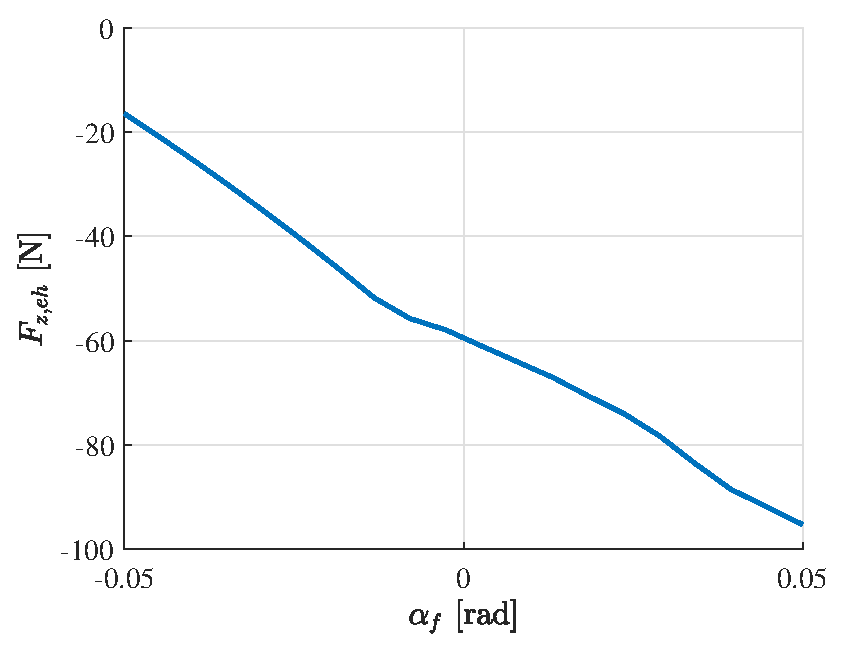
\includegraphics[width=90mm]{graficos/FEHa}
%	\caption{Fuerzas verticales (eje z cuerpo) sobre el estabilizador horizontal a distintos ángulos de ataque a nivel del mar para una velocidad de vuelo de 28 m/s.}
%	\label{FEa}
%\end{figure}
%
%\begin{figure}
%	\centering
%	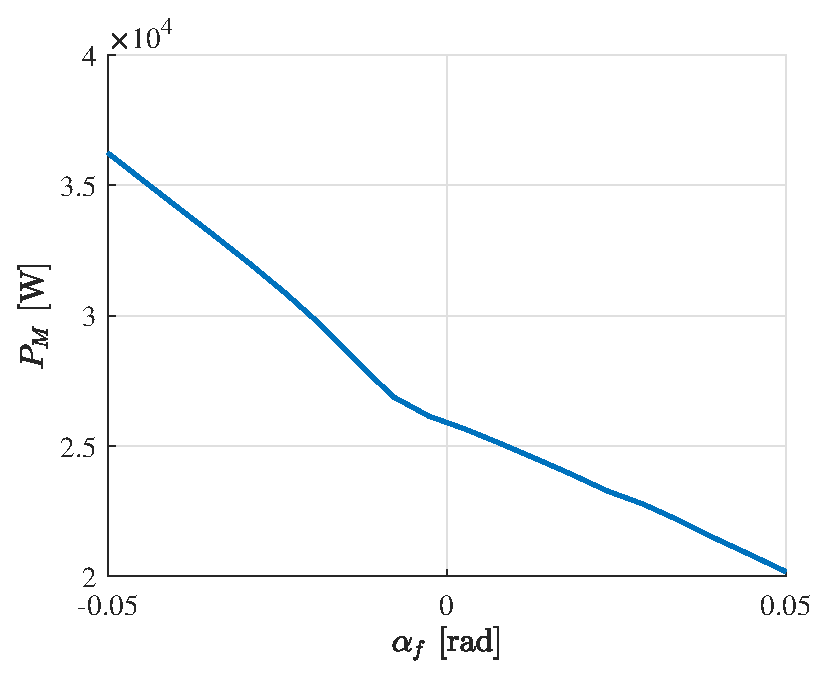
\includegraphics[width=90mm]{graficos/PMVHa}
%	\caption{Potencia necesaria para un vuelo horizontal a distintos ángulos de ataque a nivel del mar para una velocidad de vuelo de 28 m/s.}
%	\label{PMVHa}
%\end{figure}
%
%En estas circunstancias reducir el ángulo de ataque no resulta interesante, apenas variamos las cargas a costa de reducir la autonomía, pero si consideramos un vuelo con un ángulo de ataque $\alpha_f=$0.025 rad la autonomía se incrementa hasta las 5 horas y 20 minutos. Los resultados de estos cálculos se pueden encontrar en la tabla \ref{auttab2}.
%
%\begin{table}[htbp]
%	\centering
%	\begin{tabular}{|>{\columncolor{Gray}}c|c|}
%		\hline
%		\cellcolor{Gray2}Variable & \cellcolor{Gray2}Valor \\ \hline \hline
%		\cellcolor{Gray}Ángulo de ataque del fuselaje ($\alpha_f$)  & 0.025 rad \\ \hline
%		\cellcolor{Gray}Velocidad de vuelo ($V$) & 28.73 m/s \\ \hline
%		\cellcolor{Gray}Potencia necesaria ($PM$)  & 22.155 kW \\ \hline
%		\cellcolor{Gray}Consumo específico ($c_{e}$) & 9.54$\cdot$10$^-08$ kg/W$\cdot$s \\ \hline
%		\cellcolor{Gray}Autonomía ($t_{e,max}$) & 5.3231 h \\ \hline
%	\end{tabular}%
%	\caption{Parámetros relacionados con el cálculo de la autonomía del helicóptero en las condiciones de vuelo horizontal a 28.73 m/s con ángulo de ataque de 0.025 rad.}
%	\label{auttab2}
%\end{table}%
%
%\subsection{Variación de las Cargas en la Cola con el Ángulo de Resbalamiento $\boldsymbol{\beta_f}$}
%
%De manera análoga a lo hecho con el ángulo de ataque, se han calculado las variaciones de las cargas en los elementos de la cola con el ángulo de resbalamiento $\beta_f$.
%El caso del estabilizador vertical recuerda al del estabilizador horizontal del apartado anterior pero de forma inversa, la carga varía de forma casi lineal con el ángulo de resbalamiento, a mayor ángulo, menor carga (figura \ref{FEVb}). Como se ha dicho anteriormente, el estabilizador vertical ayuda a reducir la potencia necesaria para el rotor antipar, por lo que esta reducción hace necesario un nuevo cálculo de las cargas sobre el mismo. Dicho cálculo se refleja en la gráfica \ref{FAPb} y en ella se observa la tendencia esperada, las cargas aumentan con $\beta_f$, pero para comprobar si las cargas totales son menores o mayores, se ha representado en la gráfica \ref{deltafyb} que indica la variación total de las cargas horizontales debidas a estos elementos respecto a las cargas para ángulo de resbalamiento nulo.
%Esta gráfica deja claro que en lo que respecta a las cargas sobre la cola lo mas favorable es volar a ángulo de resbalamiento ligeramente positivo.  
%
%\begin{figure}
%	\centering
%	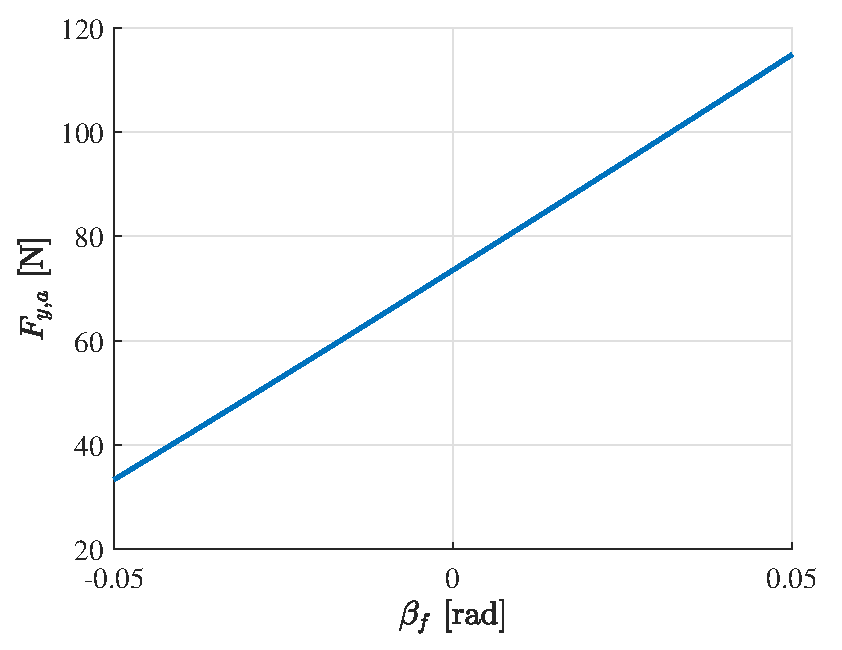
\includegraphics[width=90mm]{graficos/FAPb}
%	\caption{Fuerzas horizontales (eje y cuerpo) sobre el rotor antipar a distintos ángulos de resbalamiento a nivel del mar para un vuelo horizontal a 28 m/s.}
%	\label{FAPb}
%\end{figure}
%
%\begin{figure}
%	\centering
%	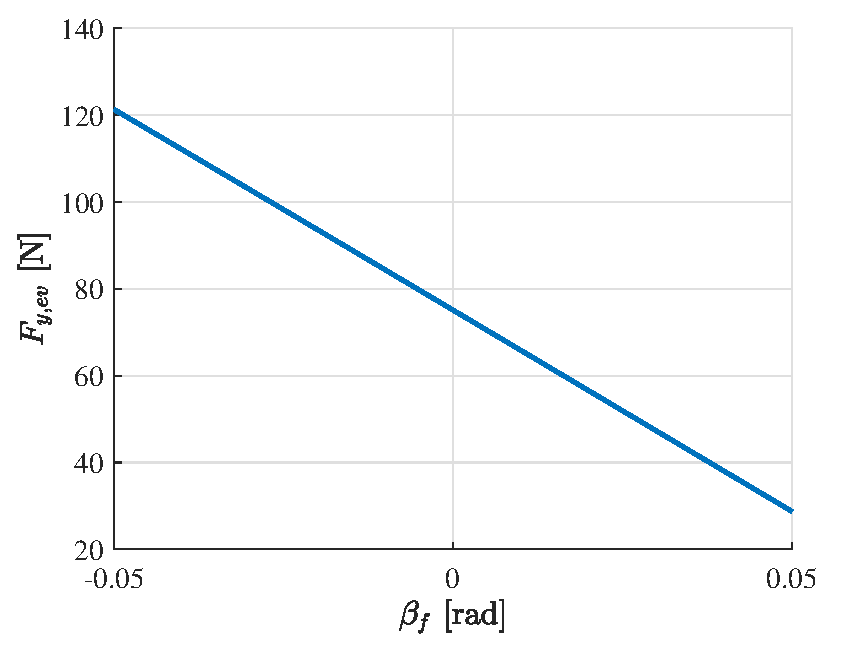
\includegraphics[width=90mm]{graficos/FEVb}
%	\caption{Fuerzas horizontales (eje y) sobre el estabilizador vertical a ángulos de resbalamiento a nivel del mar para un vuelo horizontal a 28 m/s.}
%	\label{FEVb}
%\end{figure}
%
%\begin{figure}
%	\centering
%	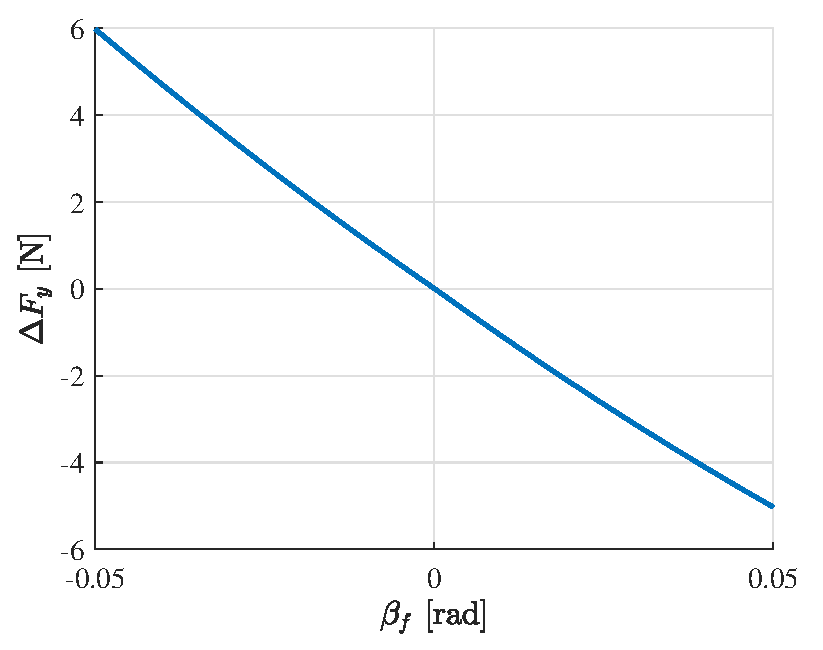
\includegraphics[width=90mm]{graficos/deltafyb}
%	\caption{Variación de la fuerza horizontal (eje y cuerpo) sobre la cola debida al estabilizador vertical y el rotor antipar a distintos ángulos de resbalamiento respecto a ángulo nulo a nivel del mar para un vuelo horizontal a 28 m/s.}
%	\label{deltafyb}
%\end{figure}
%
%\begin{figure}
%	\centering
%	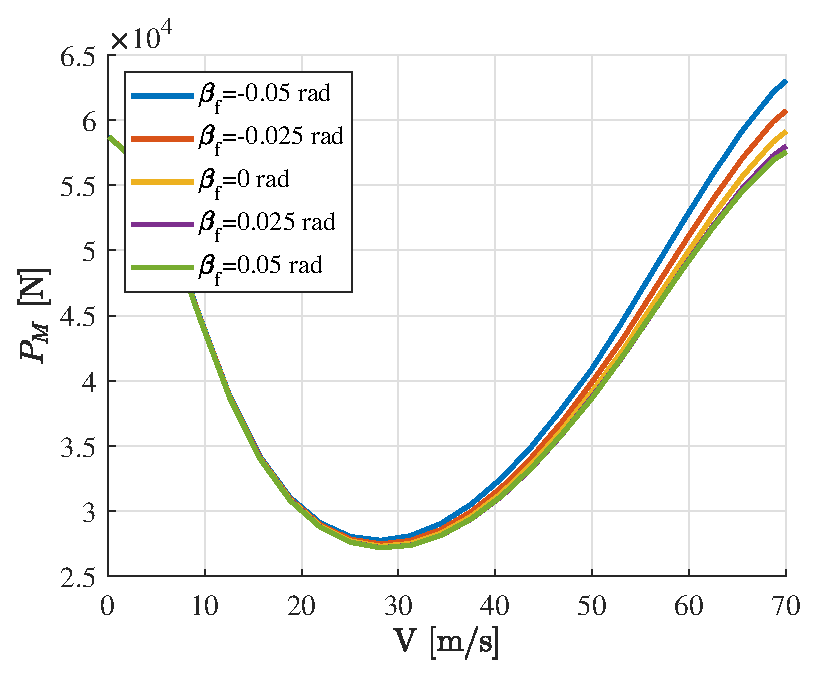
\includegraphics[width=90mm]{graficos/Potb}
%	\caption{Variación de la potencia necesaria para el vuelo horizontal a nivel del mar a distintas velocidades y ángulos de resbalamiento.}
%	\label{Potb}
%\end{figure}
%
%Para comprobar si puede resultar más eficiente volar con ángulo de resbalamiento no nulo, se ha vuelto a simular el mismo vuelo que al principio del capítulo para varios valores del ángulo de resbalamiento y los resultados de las potencias necesarias se han plasmado en la gráfica \ref{Potb} donde se observa que la potencia necesaria para el vuelo disminuye según aumenta el ángulo de resbalamiento.
%
%Todo esto indica en un primer momento que resulta mas favorable, tanto para reducir cargas como potencia necesaria, volar a pequeños ángulos de resbalamiento.
%
%Respecto al estabilizador horizontal, la gráfica \ref{FEHb} muestra que las variaciones de las cargas verticales son de 1 N como máximo, por lo que queda claro que resulta indiferente a la hora de decidir si conviene volar a un ángulo de resbalamiento u otro.
%
%
%\begin{figure}
%	\centering
%	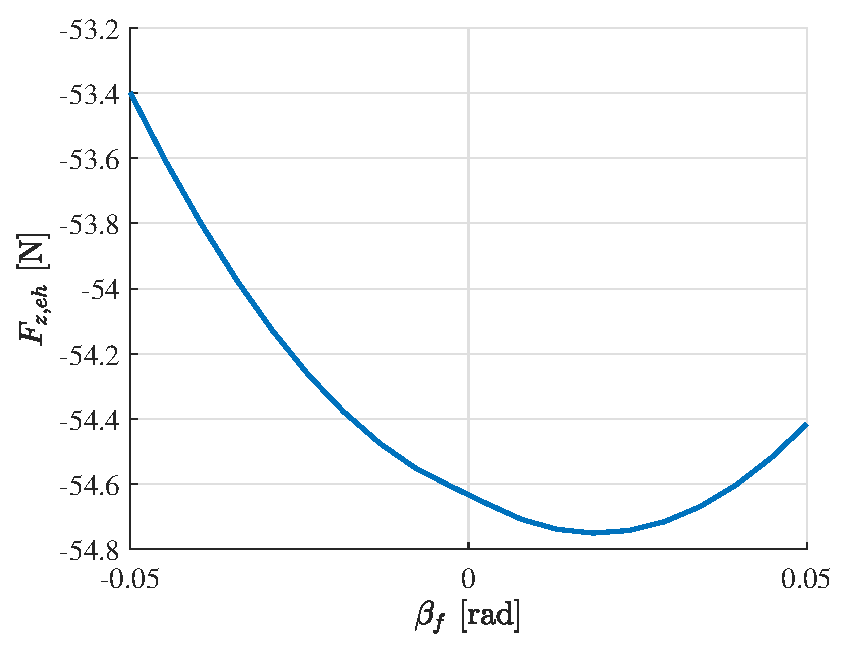
\includegraphics[width=90mm]{graficos/FEHb}
%	\caption{Fuerzas verticales (eje z cuerpo) sobre el estabilizador horizontal a ángulos de resbalamiento a nivel del mar para un vuelo horizontal a 28 m/s.}
%	\label{FEHb}
%\end{figure}

\section{Posibles Cambios en el Diseño}

Hecho un análisis de los parámetros de vuelo en distintas condiciones para el vuelo horizontal, es hora de comprobar el efecto de algunos parámetros de diseño en el vuelo. Para ello se mostrarán gráficas similares a las anteriores del mismo capítulo para diferentes valores de diferentes características de la aeronave.

\subsection{Rigidez en Batimiento $\boldsymbol{k_{\beta}}$}

Un parámetro que puede ser interesante cambiar es la rigidez de las palas en batimiento. \emph{HEROES} calcula un valor suponiendo que se quiere mantener una rigidez similar a la del rotor del helicóptero base, es decir, el Bölkow Bo 105.
Para comprobar su efecto, se ha decidido variar su valor base (denominado como $k_{\beta0}$ en las gráficas) entre el 70\% y el 130\% (tabla \ref{kbetatab}) de su valor. Los resultados de esta simulación se han reflejado en las gráficas \ref{PMVHkbeta}, \ref{ControlVHkbeta}, \ref{EulerVHkbeta} y \ref{FRPkbeta}.

\begin{table}[htbp]
	\centering
	\begin{tabular}{|>{\columncolor{Gray}}c|c|}
		\hline
		\cellcolor{Gray} & 7231.08 \\ \cline{2-2}
		\cellcolor{Gray} & 8780.6 \\ \cline{2-2}
		\cellcolor{Gray} & 10330.12 \\ \cline{2-2}
		\cellcolor{Gray} & 11879.64 \\ \cline{2-2}
		\multirow{-5}{*}{\cellcolor{Gray}$k_\beta$ (Nm/rad)} & 13429.15 \\ \hline
	\end{tabular}%
	\caption{Valores de la rigidez en batimiento de las palas usados en la simulación, en orden ascendente de valor. El valor central es el valor que \emph{HEROES} ha otorgado al modelo de forma automática.}
	\label{kbetatab}
\end{table}%

\begin{figure}
	\centering
	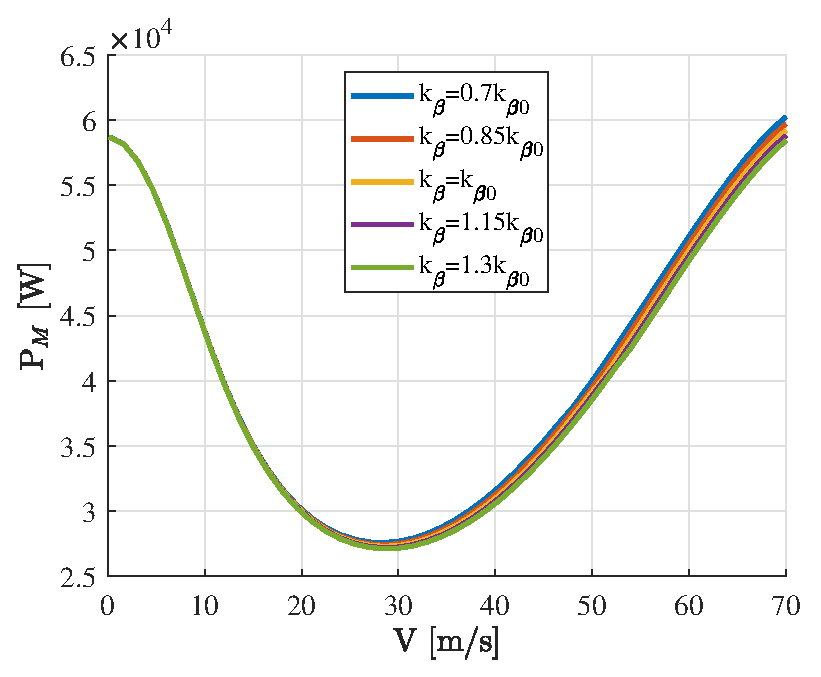
\includegraphics[width=90mm]{graficos/PMVHkbeta}
	\caption{Consumo de Potencia de la aeronave en función de la velocidad de vuelo a nivel del mar para vuelo horizontal y limitación por potencia máxima continua disponible.}
	\label{PMVHkbeta}
\end{figure}
\begin{figure}
	\centering
	\subfigure[Paso cíclico longitudinal]{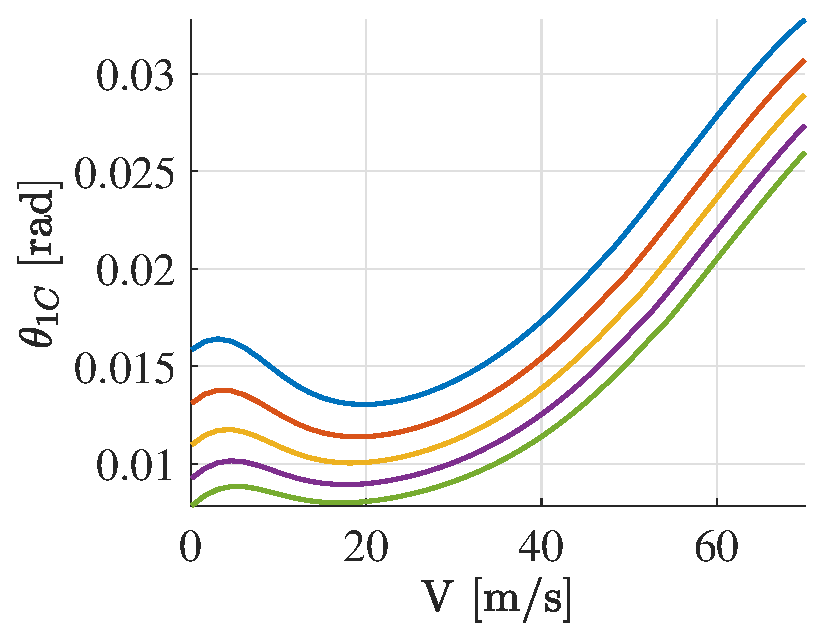
\includegraphics[width=60mm]{graficos/theta1CVHkbeta}}
	\subfigure[Paso cíclico lateral]{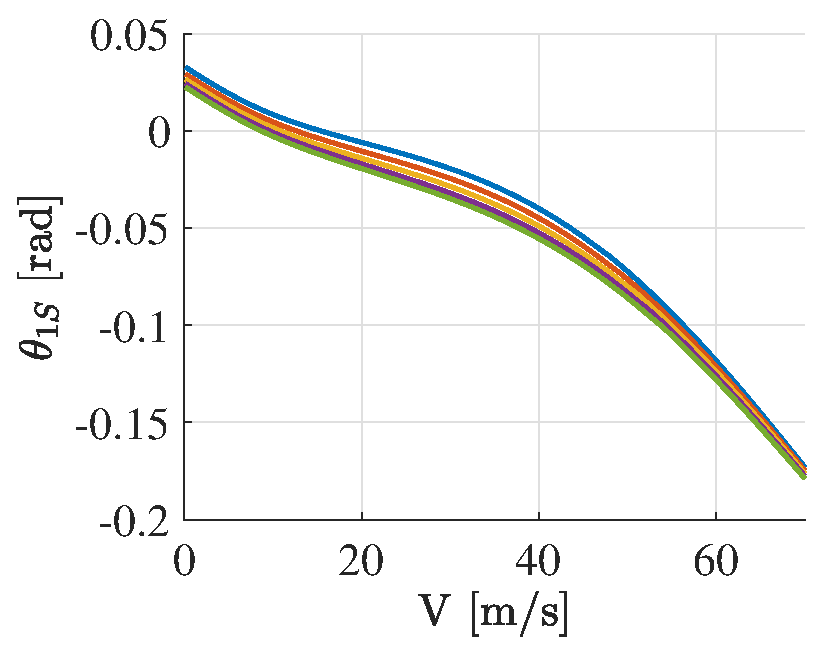
\includegraphics[width=60mm]{graficos/theta1SVHkbeta}}
	\subfigure[Paso colectivo]{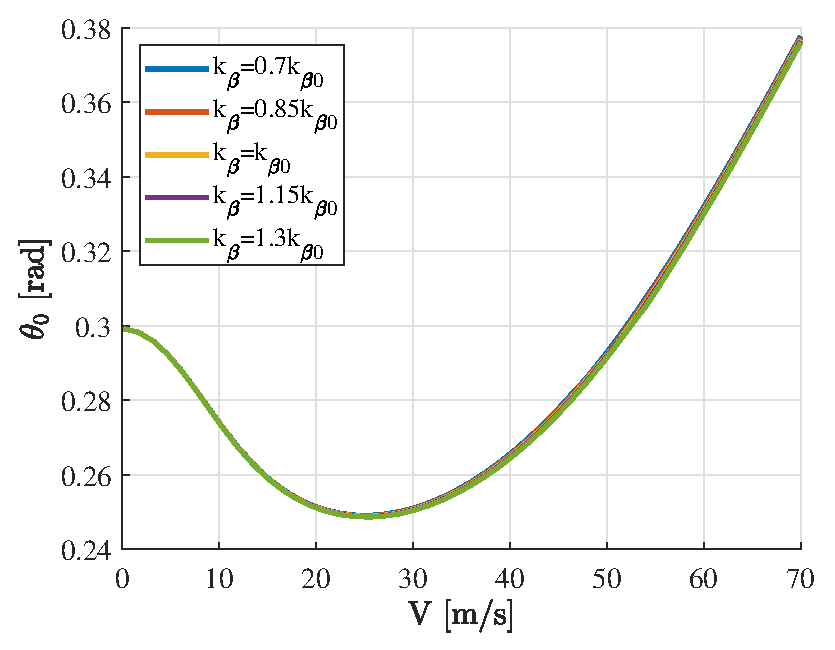
\includegraphics[width=90mm]{graficos/theta0VHkbeta}}
	\caption{Ángulos de control de la aeronave en función de la velocidad de vuelo a nivel del mar para vuelo horizontal y diferentes valores de k$_\beta$.}
	\label{ControlVHkbeta}
\end{figure}
\begin{figure}
	\centering
	\subfigure[Cabeceo]{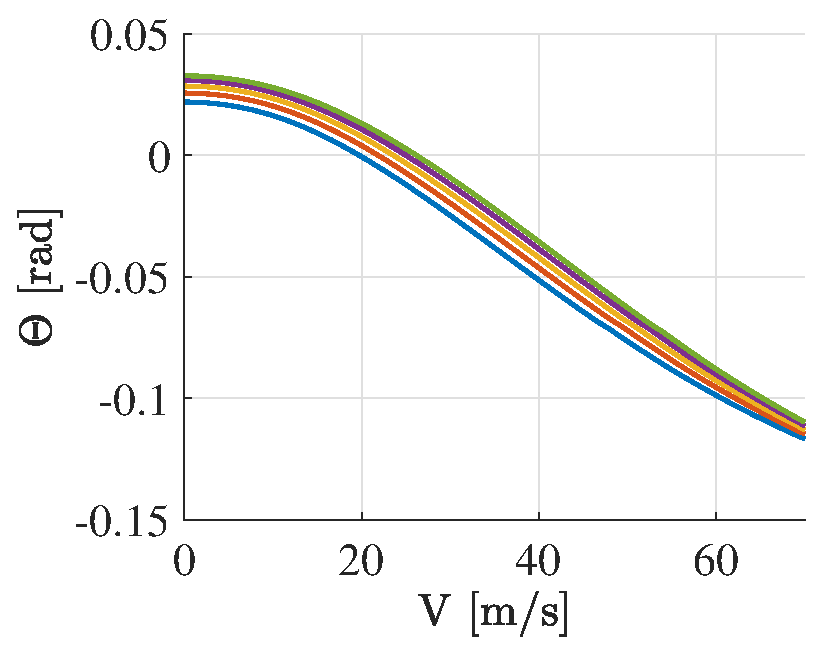
\includegraphics[width=60mm]{graficos/CabVHkbeta}}
	\subfigure[Balanceo]{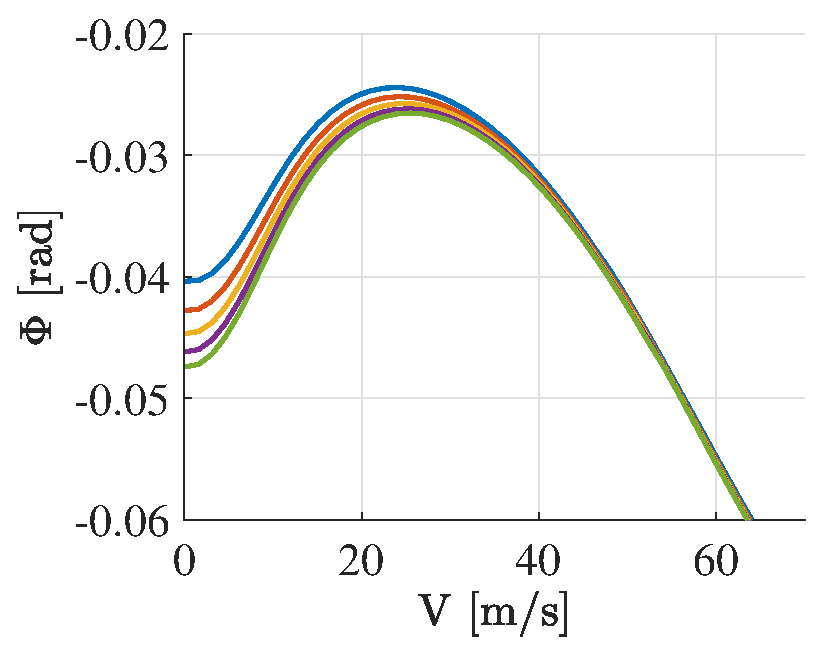
\includegraphics[width=60mm]{graficos/BalanVHkbeta}}
	\caption{Ángulos de Euler de la aeronave en función de la velocidad de vuelo a nivel del mar para vuelo horizontal y diferentes valores de k$_\beta$.}
	\label{EulerVHkbeta}
\end{figure}
\begin{figure}
	\centering
	\subfigure[Fuerzas longitudinales (eje x)]{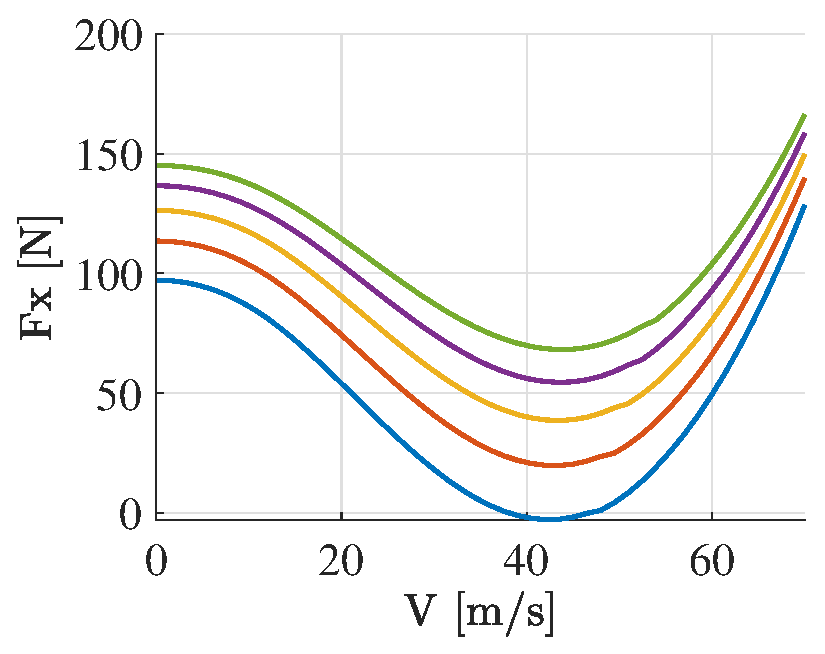
\includegraphics[width=60mm]{graficos/FRPxkbeta}}
	\subfigure[Fuerzas laterales (eje y)]{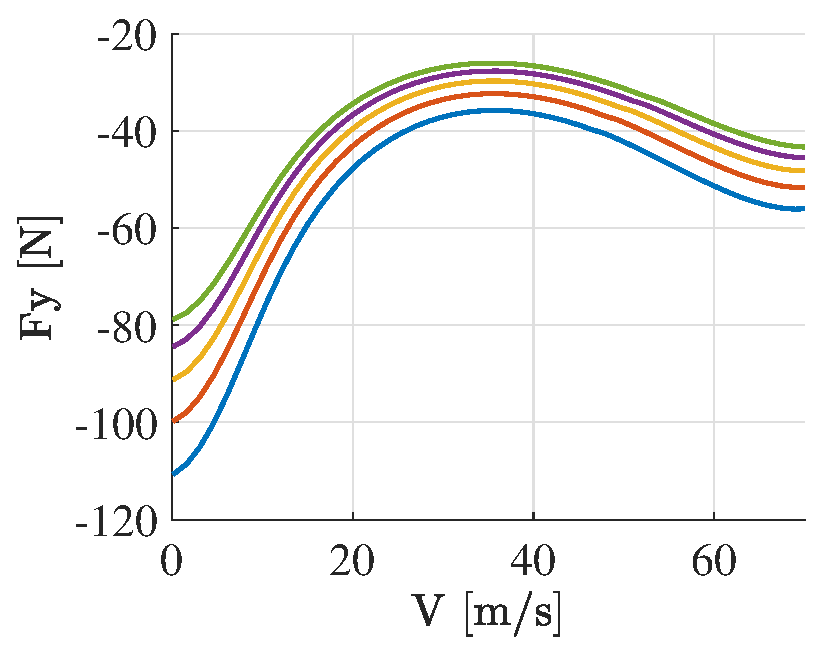
\includegraphics[width=60mm]{graficos/FRPykbeta}}
	\subfigure[Fuerzas verticales (eje z)]{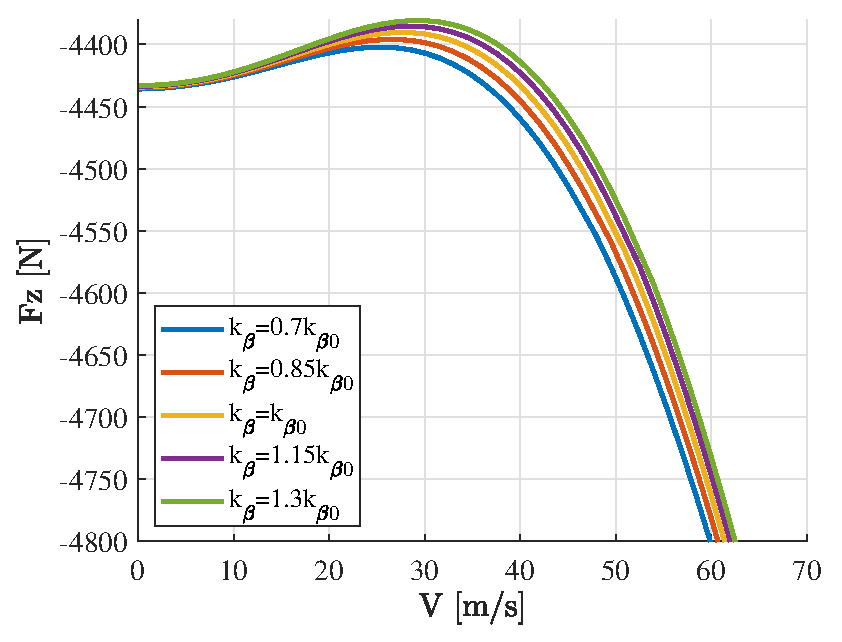
\includegraphics[width=90mm]{graficos/FRPzkbeta}}
	\caption{Fuerzas (en ejes cuerpo) sobre el rotor principal en función de la velocidad de vuelo a nivel del mar para vuelo horizontal y diferentes valores de k$_\beta$.}
	\label{FRPkbeta}
\end{figure}

Lo primero que se observa es que los cambios no son excesivamente llamativos, pero existen. En el caso de la potencia necesaria para el vuelo se observa en \ref{PMVHkbeta} que a bajas velocidades de vuelo los resultados no dependen de $k_\beta$, pero según aumenta la velocidad también lo hacen las diferencias en los resultados. Independientemente del valor de la velocidad, los resultados para una rigidez de batimiento mayor son mas favorables, es decir, la potencia necesaria para el vuelo es menor. Sin embargo, este resultado no tiene en cuenta que como consecuencia de llevar a cabo este cambio en un modelo real, las cargas sobre las palas aumentan y por tanto se han de realizar cambios también en el rotor y las palas, lo cual puede suponer aumentos de masa y de coste. En la gráfica \ref{kbetapala} se han representado el caso de máxima rigidez en batimiento anterior junto a un caso con un aumento de masa de pala de un 20\% (tabla \ref{bmtab}), lo que equivaldría a cambiar el material de fabricación de las palas para dotarlas de mayor rigidez (sin tener en cuenta posibles cambios de masa en el propio rotor). De estos resultados se observa que el aumento de masa contrarresta el efecto del aumento de rigidez, por lo que será necesario un análisis mas exhaustivo de los materiales disponibles, costes y necesidades de la aeronave para poder tomar una decisión acerca de aumentar la rigidez del rotor.

\begin{table}[htbp]
	\centering
	\begin{tabular}{|>{\columncolor{Gray}}c|c|}
		\hline
		\cellcolor{Gray}Masa de pala original & 18.798 kg \\ \hline
		\cellcolor{Gray}Masa de pala 20\% mayor & 22.558 kg \\ \hline
	\end{tabular}%
	\caption{Valores de las masas de las palas original y aumentado un 20\% suponiendo un cambio de material en su fabricación.}
	\label{bmtab}
\end{table}%

\begin{figure}
	\centering
	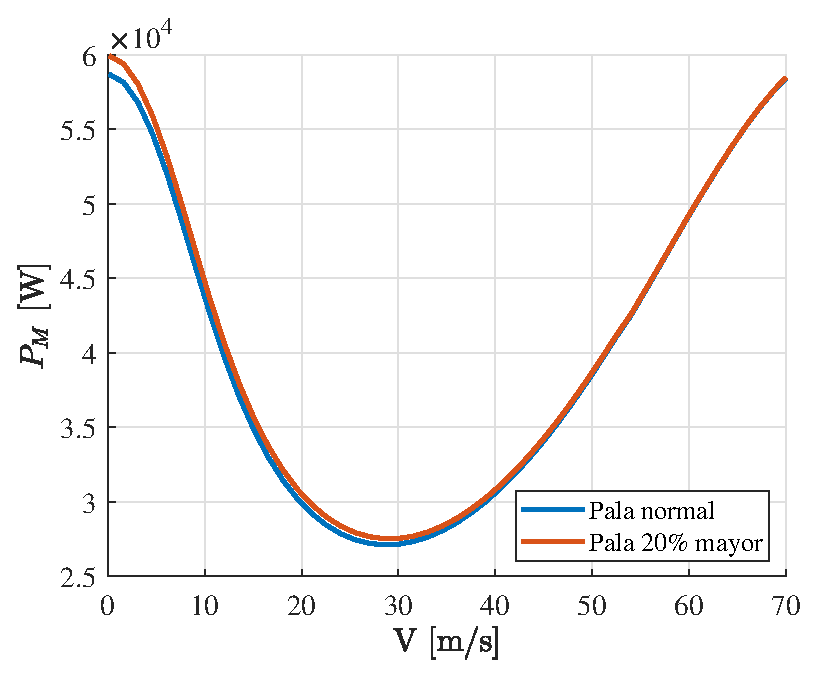
\includegraphics[width=90mm]{graficos/PMbm20}
	\caption{Potencia necesaria para un vuelo horizontal a nivel del mar a distintas velocidades de vuelo para un helicóptero de rigidez en batimiento $k_\beta$=13429.15 Nm/rad y masas de pala original y un 20\% mayor.}
	\label{kbetapala}
\end{figure}

En cuanto al resto de resultados, se puede observar en \ref{ControlVHkbeta} que el paso colectivo se mantiene prácticamente constante con $k_\beta$, por lo que los únicos cambios que se observan son en los ángulos de paso cíclico lateral y longitudinal. En ambos casos el aumento de la rigidez lleva acompañado una disminución de los ángulos de paso cíclico que en el caso del longitudinal se observa que la diferencia entre los valores máximo y mínimo de $k_\beta$ de la simulación supone alrededor de 0.005 rad, mientras que en el lateral las diferencias alcanzan valores de entre 0.01 y 0.012 rad. Estos cambios de menos de un grado son asumibles por lo que no supondría ningún problema a la hora de variar la rigidez en batimiento del rotor principal.

Donde se observan cambios mayores es en las cargas que aparecen en el rotor principal (gráfica \ref{FRPkbeta}). Lo primero que se observa es que las cargas verticales y laterales no solo no aumentan, sino que disminuyen. Las cargas verticales sufren una variación pequeña, que aumenta con la velocidad, pero esta variación llega a valores de unos 50 N a velocidades de alrededor de 40 m/s, lo que comparado con los valores de alrededor de 4475 N a los que están sometidos lo diferentes modelos a esas velocidades resulta despreciable.

En el caso de las fuerzas laterales las variaciones máximas se dan para bajas velocidades de vuelo, llegando a valores de 30 N, que a 40 m/s se ven reducidas a apenas 10 N de diferencia. Pese a que estas variaciones sean menores a las que aparecen las fuerzas verticales, su valor relativo es mucho mayor ya que los valores de las cargas son de alrededor de 100 N a velocidades muy bajas y de 35 N a 40 m/s. Esto supone una disminución importante de las cargas, al menos en el eje lateral.

Sin embargo, las cargas más críticas serían las que aparecen en el eje longitudinal del helicóptero, cuyas variaciones máximas entre las distintas configuraciones son de hasta 60 N, llegando a cargas máximas un 25\% mayores que las esperadas en el modelo original. Además el modelo más rígido sufre cargas del orden de 70 N para velocidades de vuelo en las que el modelo menos rígido no sufre ninguna carga. Estos cambios por tanto harían necesario un análisis de la estructura del rotor para comprobar si pudiese soportar las nuevas cargas o si por el contrario, conviene reducir la rigidez y con ello las cargas para reducir costes o peso.

\subsection{Integración de las Diferentes Cargas de Pago}

En el capítulo anterior se modelizaron 3 cargas de pago diferentes y se mostraron los cálculos para integrarlas en el fuselaje del helicóptero suponiendo que en todo momento se encuentran en su interior y por lo tanto no es necesario un cálculo aerodinámico. Estudiar como varían los parámetros de vuelo con la carga y su posición es importante a fin de poder realizar la integración ideal en cada caso.
Para poder comprobar como afecta la carga al vuelo, se realizarán las mismas suposiciones en las condiciones de vuelo que al principio del capítulo, sumando a ellas que en todas las configuraciones el MTOW será de 450 kg, es decir, habrá que calcular en cada carga un modelo del helicóptero cuya masa sea de 450 kg menos la masa de la propia carga de pago, para luego incorporar la carga de pago como ya se ha mostrado. De no seguir este proceso, estaríamos volando por encima del MTOW requerido en todo momento.

\begin{figure}
	\centering
	\subfigure[Potencia necesaria para el vuelo para difeerentes cargas de pago situadas en la proyección del centro de masas de la aeronave en vacío sobre el suelo.]{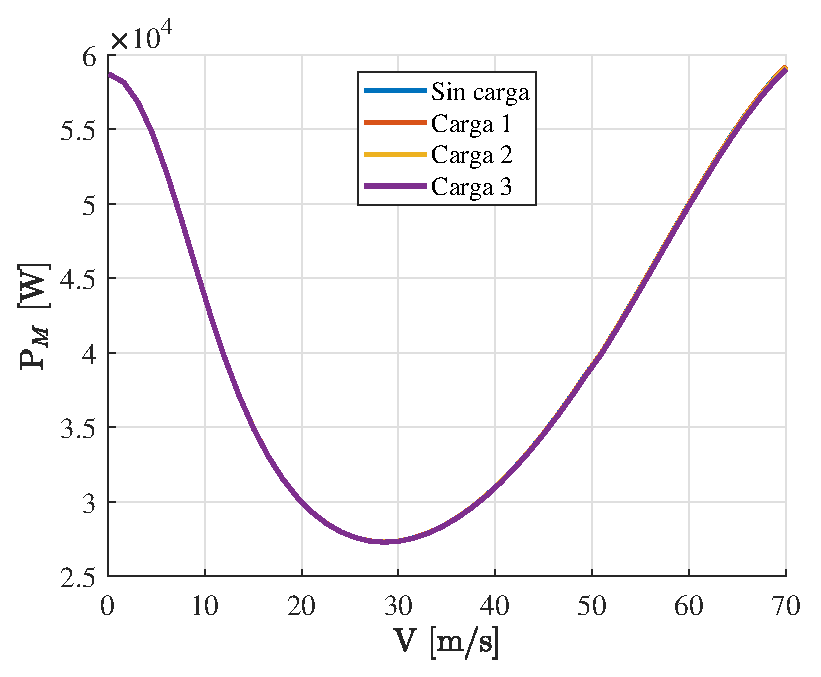
\includegraphics[width=60mm]{graficos/PMVHMPLcdg}}
	\subfigure[Potencia necesaria para el vuelo para difeerentes cargas de pago  situadas en $l_x$=1.3 m y $l_y$=-0.2 m.]{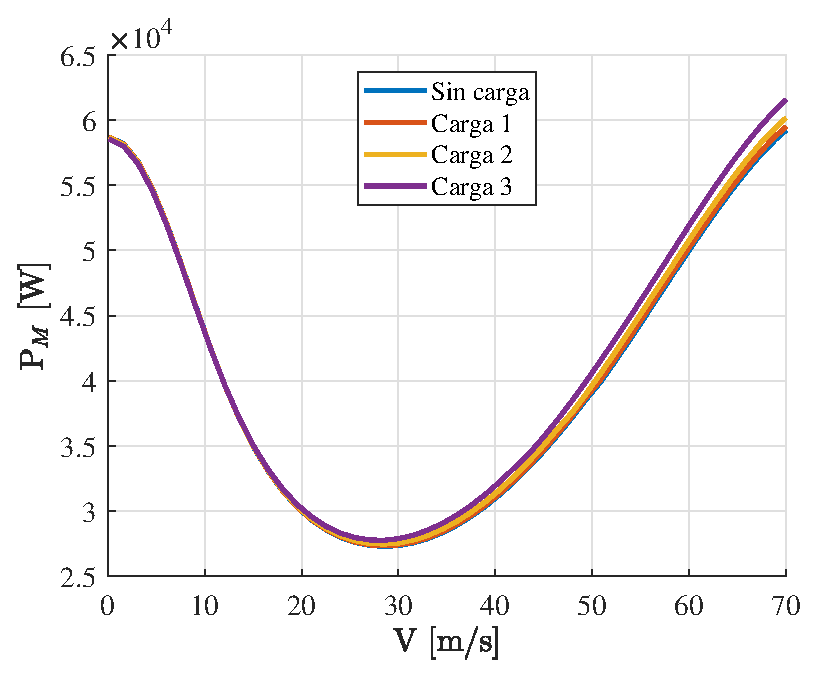
\includegraphics[width=60mm]{graficos/PMVHMPLnocdg}}
	\caption{Consumo de Potencia de la aeronave en función de la velocidad de vuelo a nivel del mar para vuelo horizontal para diferentes cargas de pago en posiciones distintas.}
	\label{PMVHMPL}
\end{figure}
\begin{figure}
	\centering
	\subfigure[Ángulo de paso colectivo del rotor principal durante el vuelo para difeerentes cargas de pago situadas en la proyección del centro de masas de la aeronave en vacío sobre el suelo.]{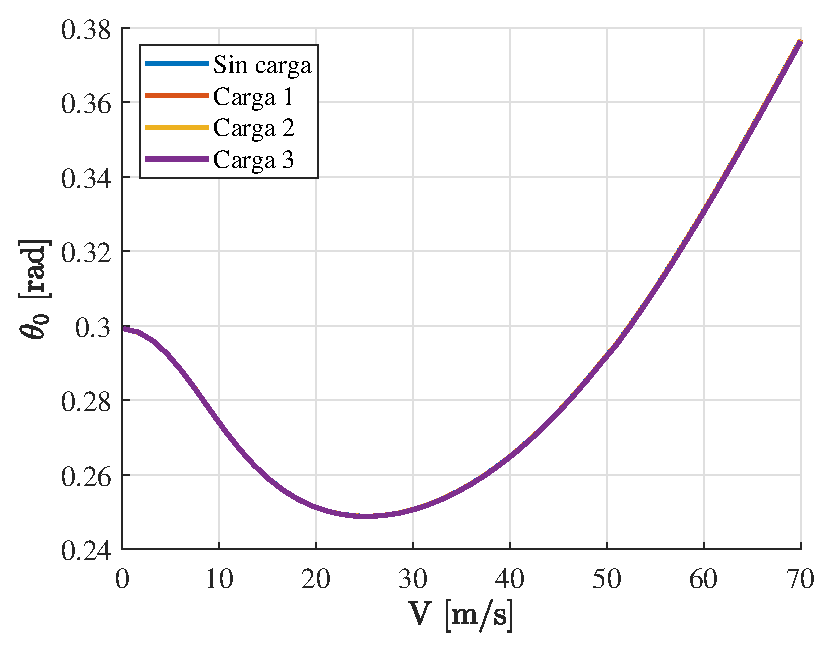
\includegraphics[width=60mm]{graficos/theta0VHMPLcdg}}
	\subfigure[Ángulo de paso colectivo del rotor principal durante el vuelo para difeerentes cargas de pago situadas en $l_x$=1.3 m y $l_y$=-0.2 m.]{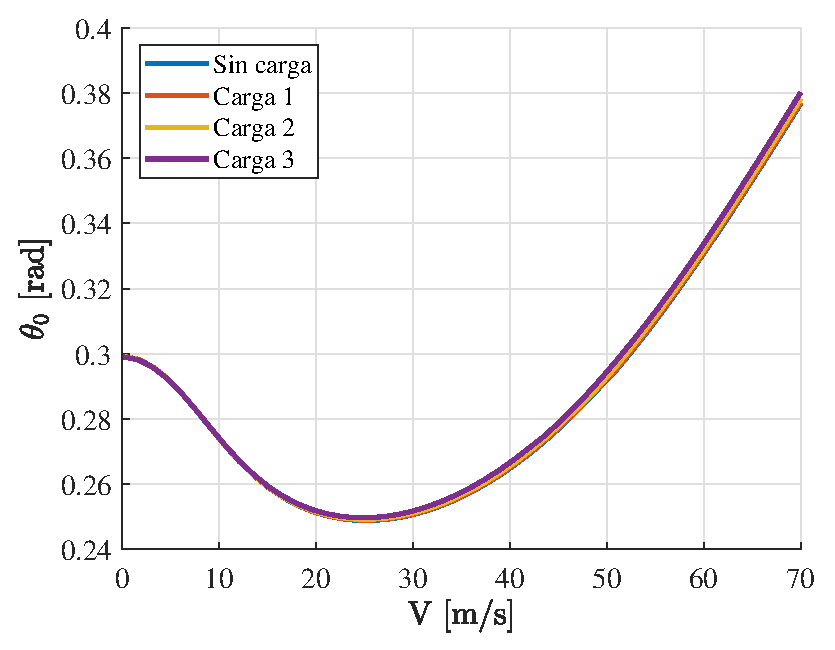
\includegraphics[width=60mm]{graficos/theta0VHMPLnocdg}}
	\caption{Ángulos de paso colectivo del rotor principal de la aeronave en función de la velocidad de vuelo a nivel del mar para vuelo horizontal para diferentes cargas de pago en posiciones distintas.}
	\label{Theta0VHMPL}
\end{figure}
\begin{figure}
	\centering
	\subfigure[Ángulo de paso cíclico longitudinal del rotor principal durante el vuelo para difeerentes cargas de pago situadas en la proyección del centro de masas de la aeronave en vacío sobre el suelo.]{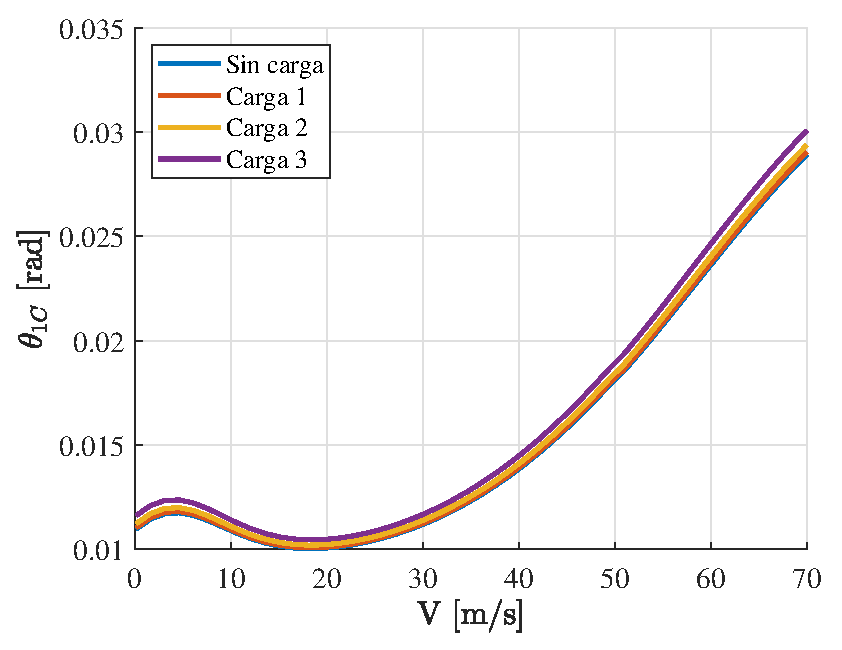
\includegraphics[width=60mm]{graficos/theta1CVHMPLcdg}}
	\subfigure[Ángulo de paso cíclico longitudinal del rotor principal durante el vuelo para difeerentes cargas de pago situadas en $l_x$=1.3 m y $l_y$=-0.2 m.]{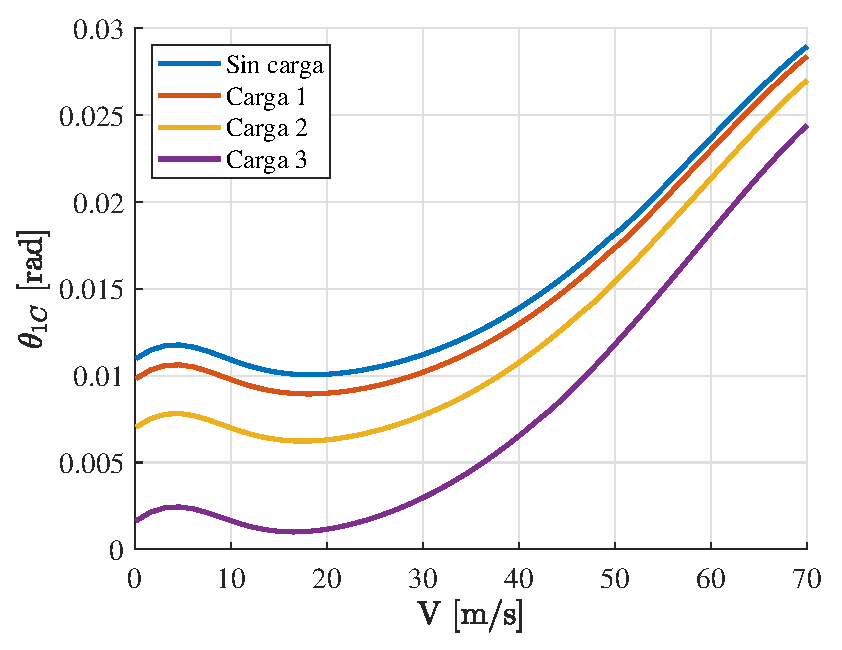
\includegraphics[width=60mm]{graficos/theta1CVHMPLnocdg}}
	\caption{Ángulos de paso cíclico longitudinal del rotor principal de la aeronave en función de la velocidad de vuelo a nivel del mar para vuelo horizontal para diferentes cargas de pago en posiciones distintas.}
	\label{Theta1CVHMPL}
\end{figure}
\begin{figure}
	\centering
	\subfigure[Ángulo de paso cíclico lateral del rotor principal durante el vuelo para difeerentes cargas de pago situadas en la proyección del centro de masas de la aeronave en vacío sobre el suelo.]{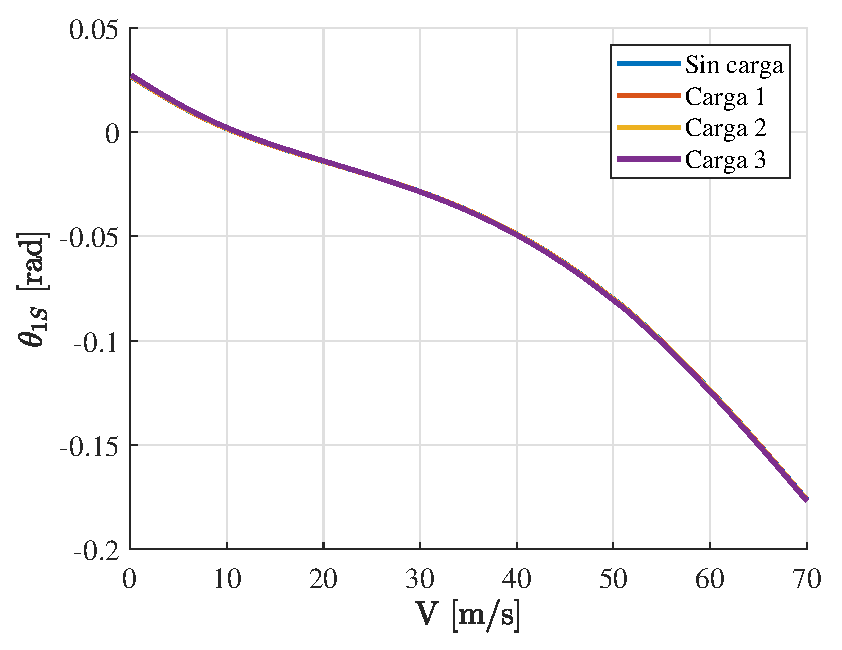
\includegraphics[width=60mm]{graficos/theta1SVHMPLcdg}}
	\subfigure[Ángulo de paso cíclico lateral del rotor principal durante el vuelo para difeerentes cargas de pago situadas en $l_x$=1.3 m y $l_y$=-0.2 m.]{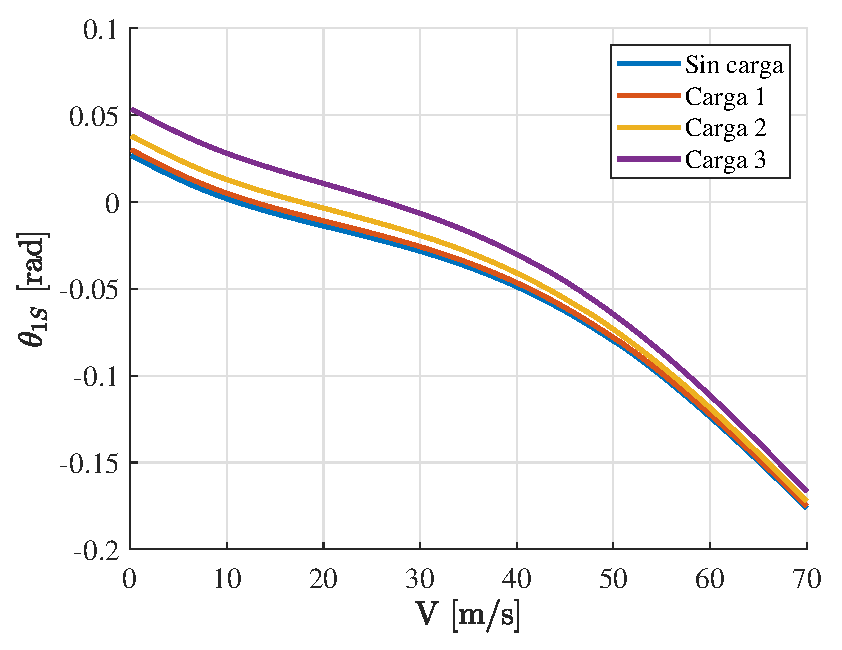
\includegraphics[width=60mm]{graficos/theta1SVHMPLnocdg}}
	\caption{Ángulos de paso cíclico lateral del rotor principal de la aeronave en función de la velocidad de vuelo a nivel del mar para vuelo horizontal para diferentes cargas de pago en posiciones distintas.}
	\label{Theta1SVHMPL}
\end{figure}
\begin{figure}
	\centering
	\subfigure[Ángulo de cabeceo de la aeronave durante el vuelo para difeerentes cargas de pago situadas en la proyección del centro de masas de la aeronave en vacío sobre el suelo.]{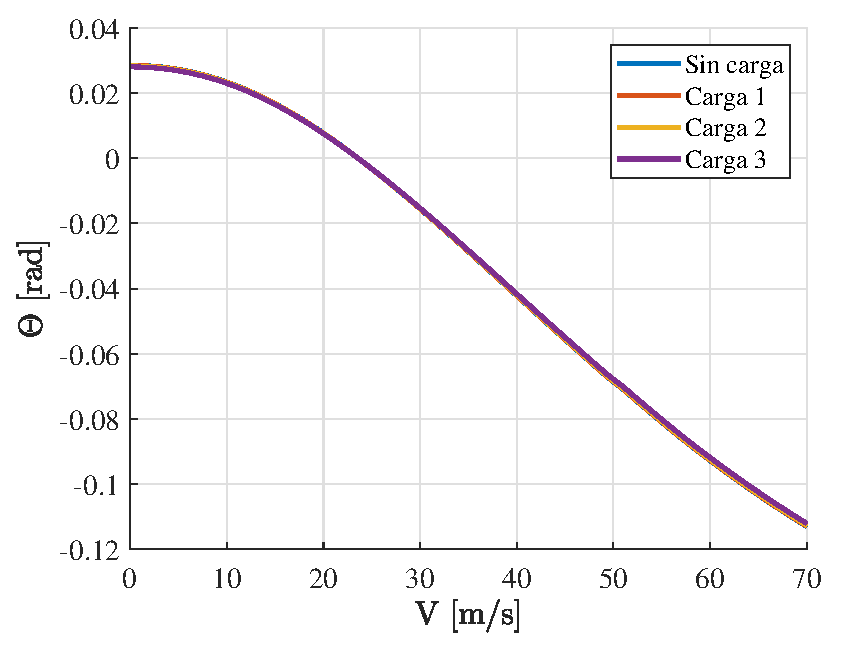
\includegraphics[width=60mm]{graficos/CabVHMPLcdg}}
	\subfigure[Ángulo de cabeceo de la aeronave durante el vuelo para difeerentes cargas de pago situadas en $l_x$=1.3 m y $l_y$=-0.2 m.]{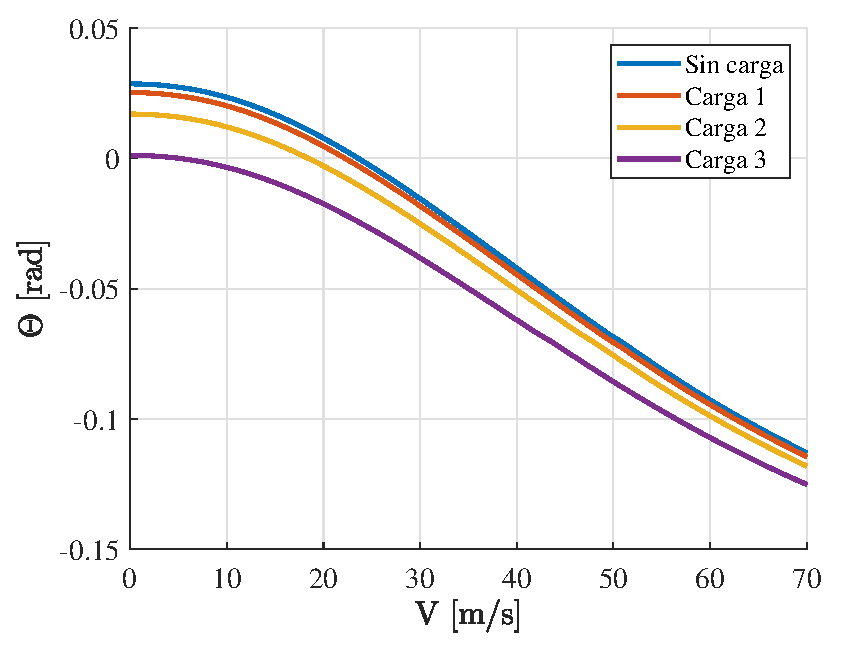
\includegraphics[width=60mm]{graficos/CabVHMPLnocdg}}
	\caption{Ángulos de cabeceo de la aeronave en función de la velocidad de vuelo a nivel del mar para vuelo horizontal para diferentes cargas de pago en posiciones distintas.}
	\label{ThetaVHMPL}
\end{figure}
\begin{figure}
	\centering
	\subfigure[Ángulo de balanceo de la aeronave durante el vuelo para difeerentes cargas de pago situadas en la proyección del centro de masas de la aeronave en vacío sobre el suelo.]{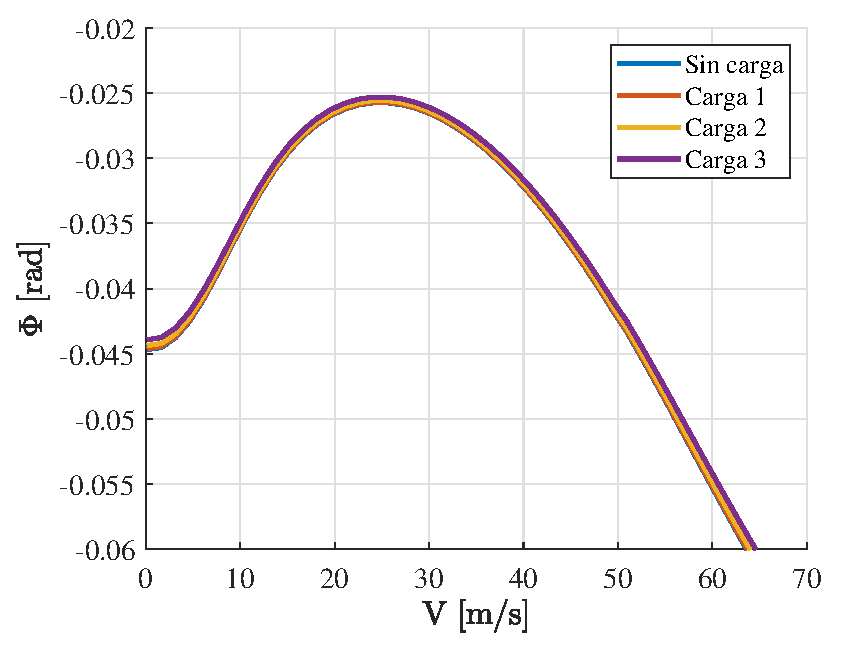
\includegraphics[width=60mm]{graficos/BalanVHMPLcdg}}
	\subfigure[Ángulo de balanceo de la aeronave durante el vuelo para difeerentes cargas de pago situadas en $l_x$=1.3 m y $l_y$=-0.2 m.]{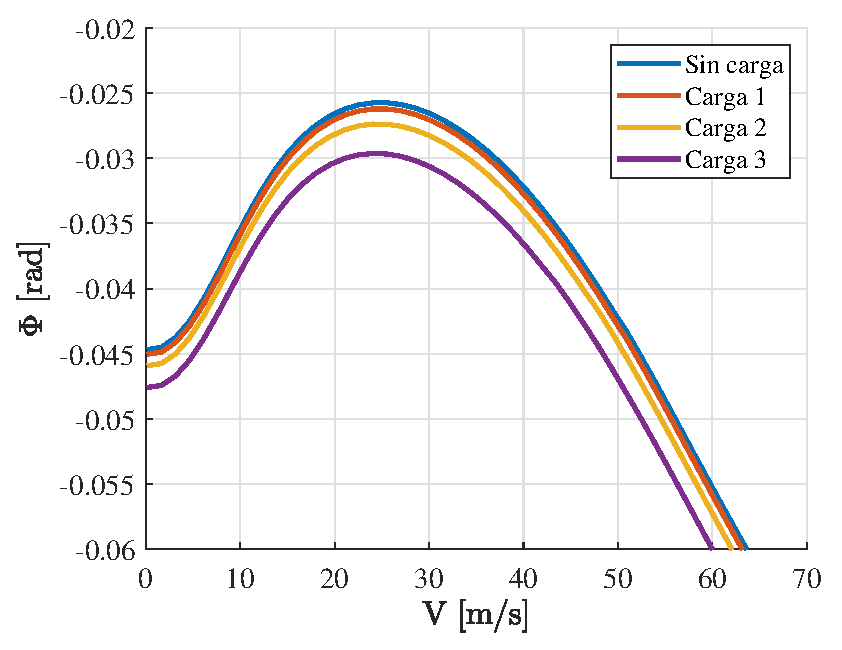
\includegraphics[width=60mm]{graficos/BalanVHMPLnocdg}}
	\caption{Ángulos de balanceo de la aeronave en función de la velocidad de vuelo a nivel del mar para vuelo horizontal para diferentes cargas de pago en posiciones distintas.}
	\label{PhiVHMPL}
\end{figure}
\begin{figure}
	\centering
	\subfigure[Ángulo de paso colectivo del rotor antipar durante el vuelo para difeerentes cargas de pago situadas en la proyección del centro de masas de la aeronave en vacío sobre el suelo.]{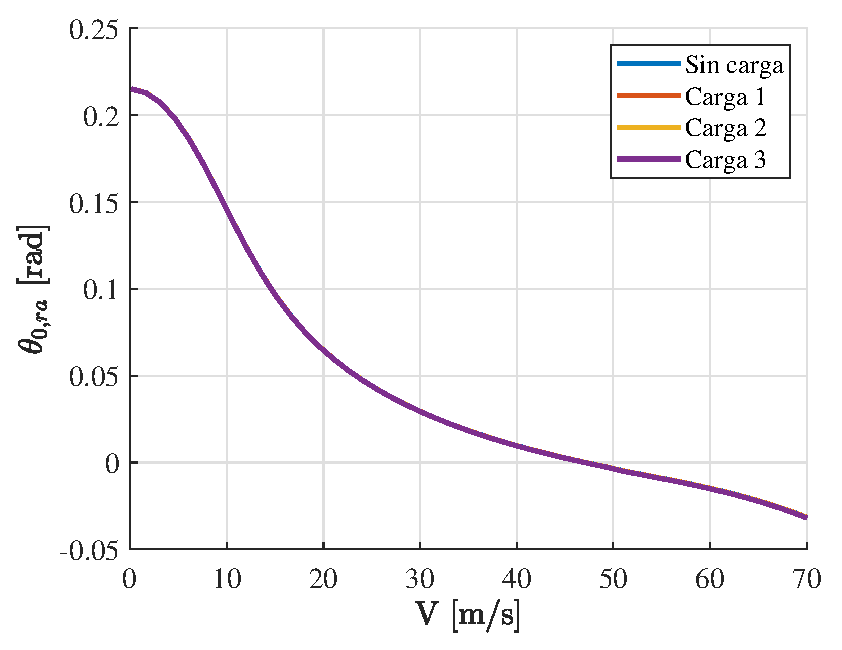
\includegraphics[width=60mm]{graficos/theta0VHraMPLcdg}}
	\subfigure[Ángulo de paso colectivo del rotor antipar durante el vuelo para difeerentes cargas de pago situadas en $l_x$=1.3 m y $l_y$=-0.2 m.]{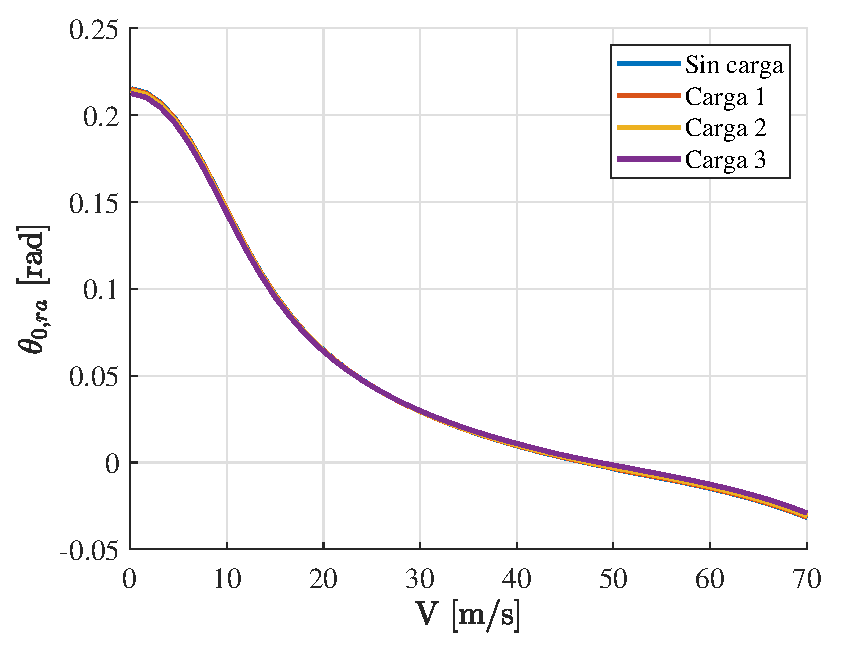
\includegraphics[width=60mm]{graficos/theta0VHraMPLnocdg}}
	\caption{Ángulos de paso colectivo del rotor antipar de la aeronave en función de la velocidad de vuelo a nivel del mar para vuelo horizontal para diferentes cargas de pago en posiciones distintas.}
	\label{Theta0VHraMPL}
\end{figure}

Las simulaciones se han realizado para las configuraciones sin carga y para cada una de las cargas en dos posiciones, sobre la proyección del centro de masas del helicóptero sin la carga sobre el suelo y para una posición de la carga en en suelo tal que $l_x$=1.3 m y $l_y$=-0.2 m, es decir, con las cámaras situadas en la parte delantera del helicóptero y desviadas ligeramente hacia un lateral del fuselaje. Los resultados de estas simulaciones se han reflejado en las gráficas \ref{PMVHMPL}, \ref{Theta0VHMPL}, \ref{Theta1CVHraMPL}, \ref{Theta1SVHMPL}, \ref{ThetaVHMPL}, \ref{PhiVHMPL} y \ref{Theta0VHraMPL}.

De los resultados se puede apreciar que en caso de colocar la carga de pago sobre la proyección las condiciones de vuelo apenas varían, por lo que los cálculos realizados para la configuración sin carga en vuelo horizontal se pueden asumir que sirven como aproximaciones para cualquier carga de las ensayadas siempre y cuando esté situada en ese punto.

Los resultados mas interesantes se dan cuando la carga se desplaza de dicho punto, siendo los casos más desfavorables los de mayor masa de carga de pago. En la gráfica \ref{PMVHMPL} se observa que a bajas velocidades de vuelo las diferencias son inapreciables, pero al aumentar la misma, lo hacen también las diferencias. Aún así, las diferencias en las potencias necesarias no son excesivas, llegando a valores de cerca de 2000 W para velocidades de 60 m/s.

En lo que respecta al ángulo de paso colectivo del rotor principal, al ser una configuración muy similar a la original y tener que sustentar el mismo peso, apenas varía con la carga ni la velocidad como se puede apreciar en la gráfica \ref{Theta0VHMPL}. Diferente es el caso de los ángulos de paso cíclico, tanto longitudinal como lateral. En el caso del ángulo de paso cíclico longitudinal, se ve en la gráfica \ref{Theta1CVHMPL} que a mayor carga, menor es su valor. Esto se explica fácilmente al observar la posición de la carga; una carga en la zona frontal del helicóptero adelantará el centro de masas del mismo, lo que contribuye a disminuir el ángulo de cabeceo (gráfica \ref{ThetaVHMPL}) y, por tanto, la necesidad de un ángulo de paso cíclico longitudinal que permita el vuelo en avance. Si el fuselaje tiene un ángulo de cabeceo tal que la perpendicular al plano del rotor tenga la dirección de avance, no es necesario un paso cíclico que redirija la fuerza en esa dirección.

Con el ángulo de paso cíclico lateral pasa algo similar, el desequilibrio másico que supone colocar una carga en una posición desplazada lateralmente del centro de masas del helicóptero provoca una variación en el ángulo de balanceo del vehículo (gráfica \ref{PMVHMPL}) que en este caso contribuye al desequilibrio ya existente, por lo que el paso cíclico lateral necesario para poder mantener la aeronave en equilibrio aumenta, al contrario de lo que pasaba con el paso longitudinal.

Por último se ha representado en la gráfica \ref{Theta0VHraMPL} la variación del ángulo de paso colectivo del rotor antipar necesario para equilibrar cada uno de los casos descritos, pero al igual que pasaba con el del rotor principal, no sufre cambios excesivos.

\subsection*{Análisis de los Parámetros de Vuelo con la Posición de la Carga de Pago}

Visto el efecto de la propia carga sobre los parámetros de vuelo, conviene comprobar el efecto de la posición de una misma carga volando a una velocidad determinada, por lo que en este apartado se reflejarán y comentarán los resultados de simular vuelos horizontales a velocidad constante para las cargas 2 y 3 en función de la posición de la misma dentro de los márgenes establecidos en el capítulo anterior.

Como comentario general, se puede observar que el cambio de la carga apenas influye en los efectos de su posición, variando ligeramente eso si las diferentes características a analizar.

\begin{figure}
	\centering
	\subfigure[Potencia necesaria para el vuelo en función de la posición relativa a $O_f$ de la carga 2 para una velocidad de vuelo de 10 m/s.]{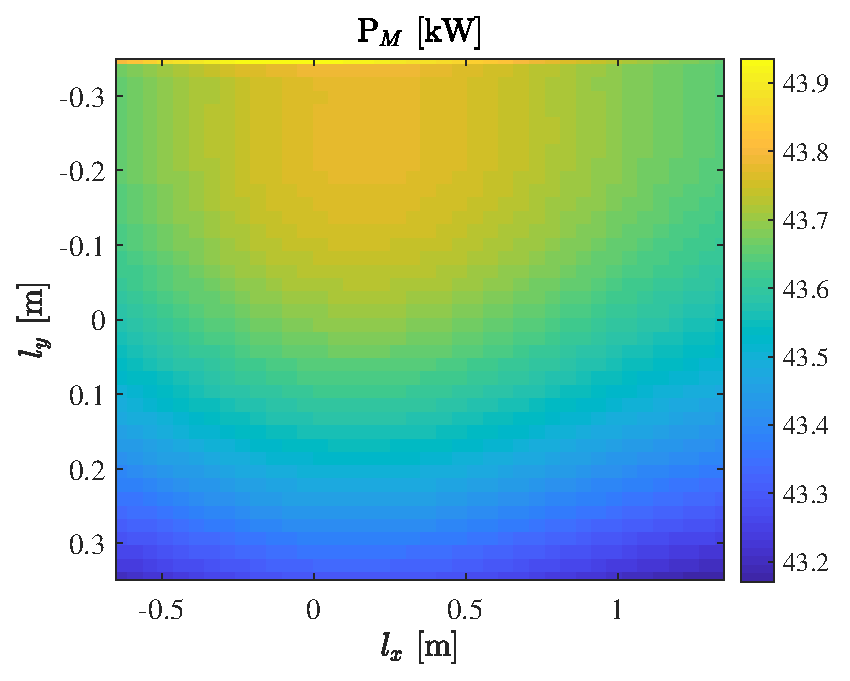
\includegraphics[width=60mm]{graficos/PMVH2lxy10ms}}
	\subfigure[Potencia necesaria para el vuelo en función de la posición relativa a $O_f$ de la carga 2 para una velocidad de vuelo de 50 m/s.]{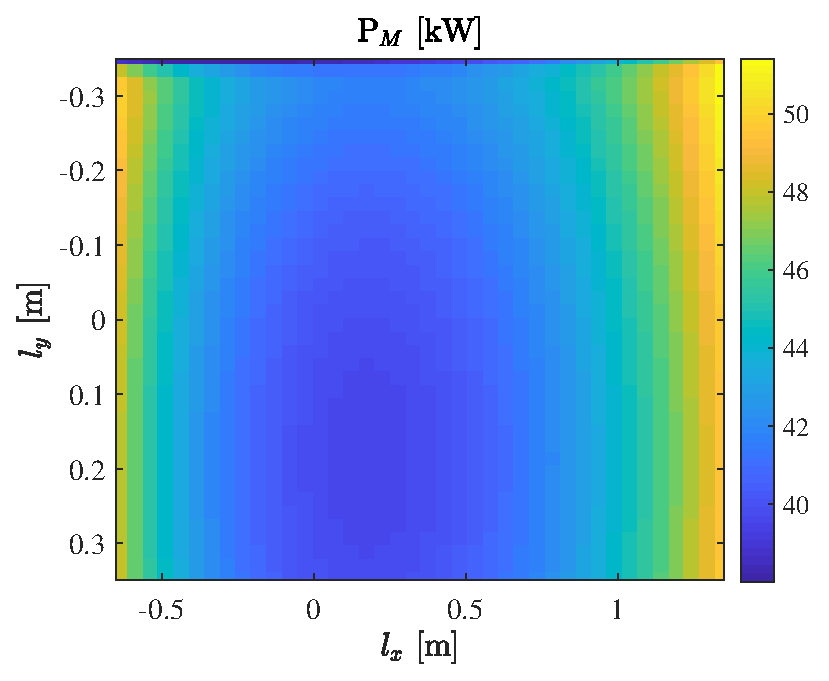
\includegraphics[width=60mm]{graficos/PMVH2lxy50ms}}
	\caption{Consumo de Potencia de la aeronave en función de la posición relativa a $O_f$ de la carga 2.}
	\label{PMVH2lxy}
\end{figure}
\begin{figure}
	\centering
	\subfigure[Potencia necesaria para el vuelo en función de la posición relativa a $O_f$ de la carga 3 para una velocidad de vuelo de 10 m/s.]{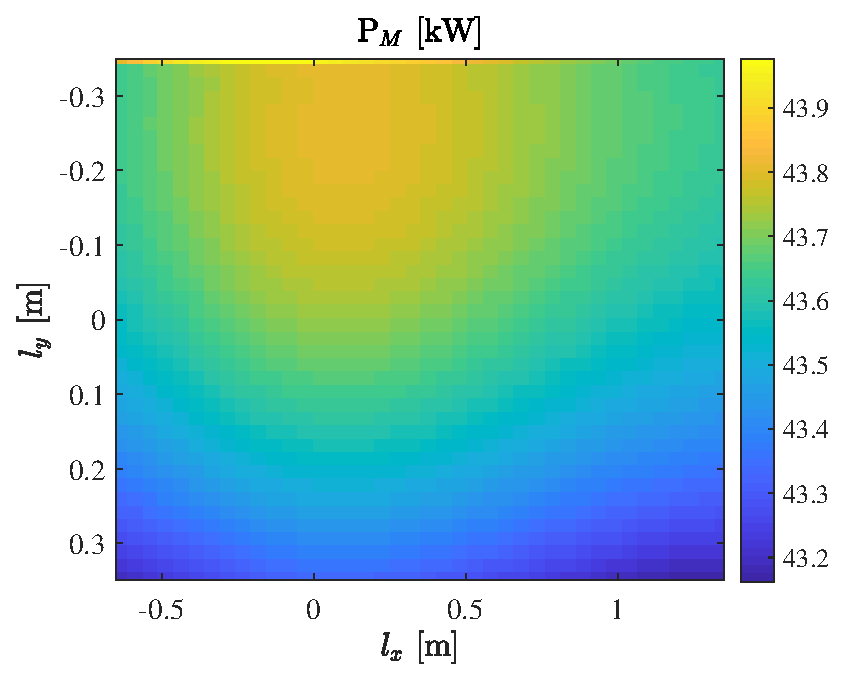
\includegraphics[width=60mm]{graficos/PMVH3lxy10ms}}
	\subfigure[Potencia necesaria para el vuelo en función de la posición relativa a $O_f$ de la carga 3 para una velocidad de vuelo de 50 m/s.]{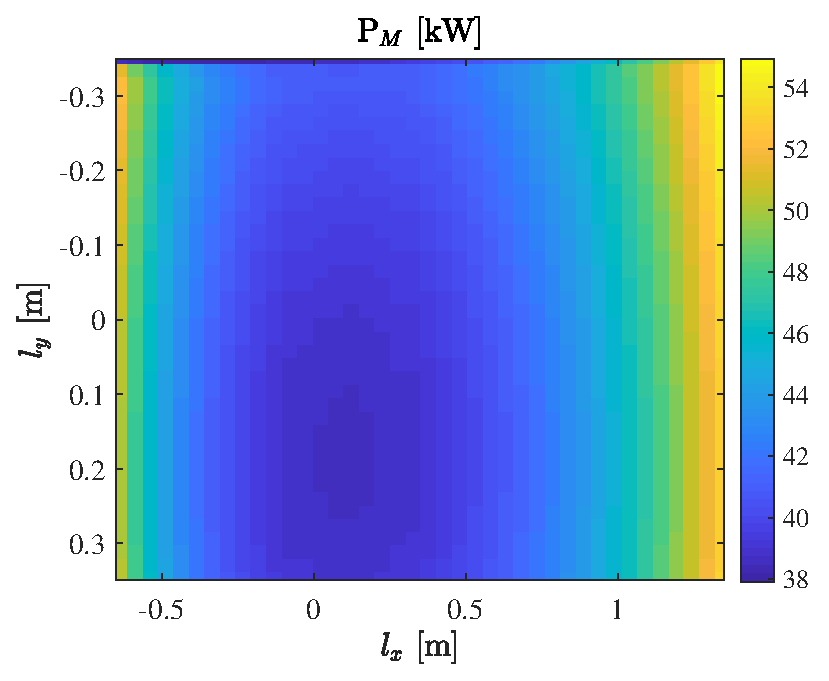
\includegraphics[width=60mm]{graficos/PMVH3lxy50ms}}
	\caption{Consumo de Potencia de la aeronave en función de la posición relativa a $O_f$ de la carga 3.}
	\label{PMVH3lxy}
\end{figure}

Comenzando por la potencia, los resultado resultan bastante curiosos; las gráficas \ref{PMVH2lxy} y \ref{PMVH3lxy} muestran que a bajas velocidades la potencia necesaria para el vuelo aumenta según disminuye $l_y$, es decir, es mayor cuanto mas a la izquierda del fuselaje esté situada la carga y también aumenta para cargas alejadas longitudinalmente del centro de gravedad de la aeronave sin carga ($x_{CG}=0.0972$). Sin embargo, a altas velocidades este comportamiento se invierte para el eje longitudinal, siendo los puntos de menor consumo aquellos en los que la carga está situada sobre el centro de gravedad de la aeronave. En el eje lateral, vuelve a repetirse el mismo comportamiento, la potencia necesaria disminuye para cargas situadas hacia la derecha del fuselaje, pero en esta ocasión aparece un mínimo alrededor de $l_y=0.2$, por lo que desplazar aún más la carga resulta perjudicial en términos de potencia. Además, a estas velocidades, estos cambios pueden suponer una reducción de hasta 10 kW respecto a valores extremos de posición, a diferencia de a bajas velocidades donde las diferencias apenas alcanzan el valor de 1 kW.

Comparando los efectos de ambas cargas, se observa que a bajas velocidades su comportamiento es prácticamente idéntico, pero a altas velocidades las cargas más pesadas y de mayor tamaño requieren de un consumo ligeramente mayor de potencia en posiciones distintas de la óptima.

\begin{figure}
	\centering
	\subfigure[Ángulo de paso colectivo del rotor principal en función de la posición relativa a $O_f$ de la carga 2 para una velocidad de vuelo de 10 m/s.]{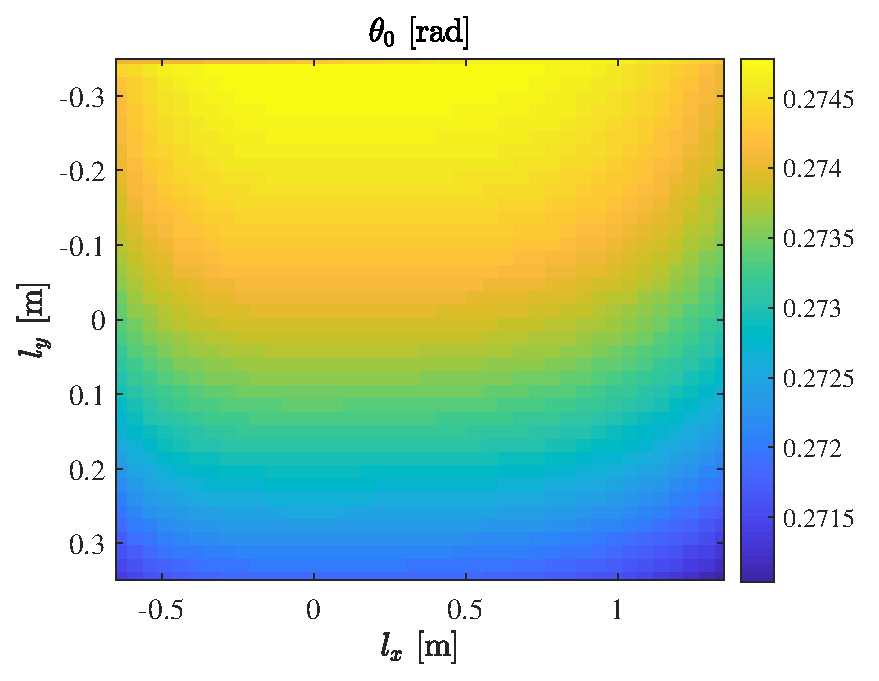
\includegraphics[width=60mm]{graficos/theta0VH2lxy10ms}}
	\subfigure[Ángulo de paso colectivo del rotor principal en función de la posición relativa a $O_f$ de la carga 2 para una velocidad de vuelo de 50 m/s.]{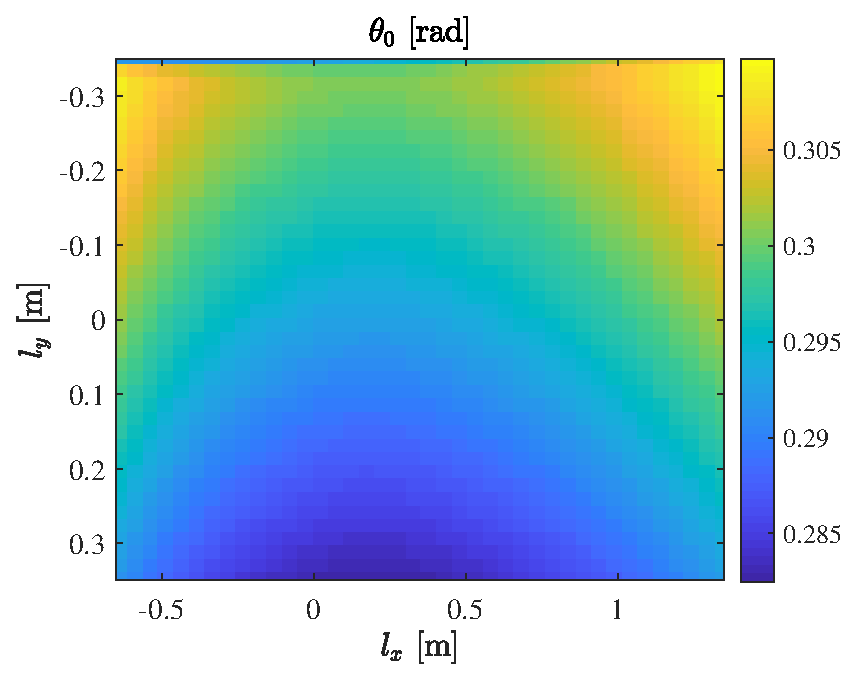
\includegraphics[width=60mm]{graficos/theta0VH2lxy50ms}}
	\caption{Ángulo de paso colectivo del rotor principal en función de la posición relativa a $O_f$ de la carga 2.}
	\label{theta0VH2lxy}
\end{figure}
\begin{figure}
	\centering
	\subfigure[Ángulo de paso colectivo del rotor principal en función de la posición relativa a $O_f$ de la carga 3 para una velocidad de vuelo de 10 m/s.]{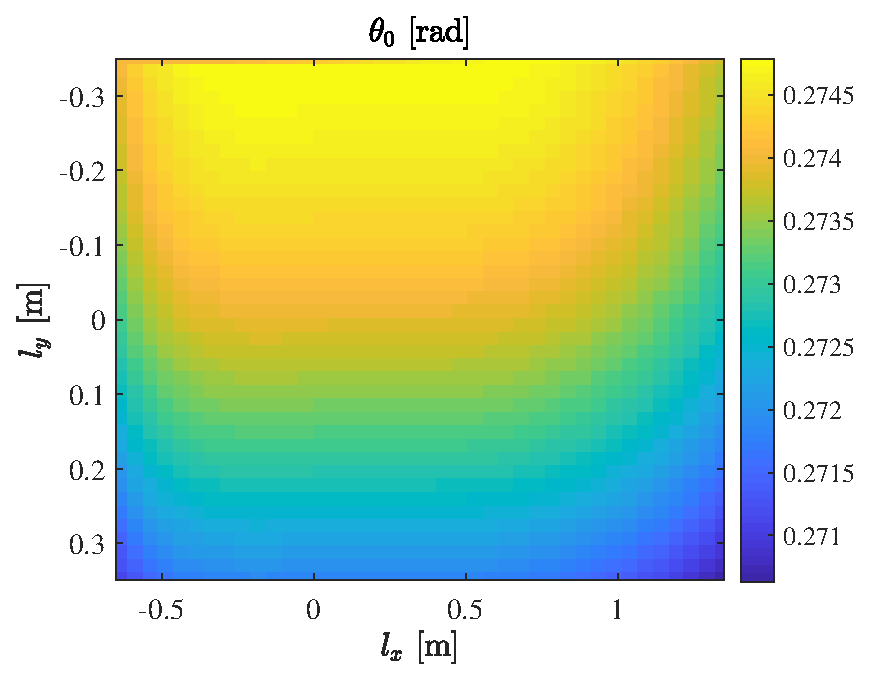
\includegraphics[width=60mm]{graficos/theta0VH3lxy10ms}}
	\subfigure[Ángulo de paso colectivo del rotor principal en función de la posición relativa a $O_f$ de la carga 3 para una velocidad de vuelo de 50 m/s.]{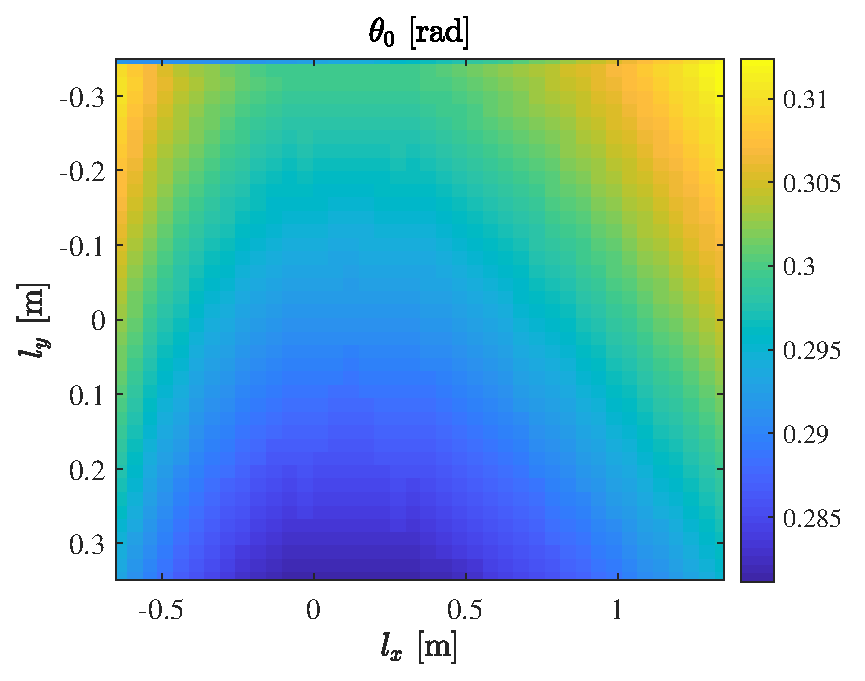
\includegraphics[width=60mm]{graficos/theta0VH3lxy50ms}}
	\caption{Ángulo de paso colectivo del rotor principal en función de la posición relativa a $O_f$ de la carga 3.}
	\label{theta0VH3lxy}
\end{figure}

En lo referente a los ángulos de control del rotor principal, de nuevo se observa en las gráficas \ref{theta0VH2lxy} y \ref{theta0VH3lxy} diferencias para altas y bajas velocidades, al menos en el paso colectivo. A bajas velocidades, el paso colectivo es menor para cargas situadas en los márgenes longitudinales y a la derecha del fuselaje, pero a altas velocidades el efecto de la posición longitudinal vuelve a invertirse, resultando necesarios pasos menores en cargas centradas. En este caso los valores para las diferentes cargas son muy similares, no existe una diferencia apreciable debido al efecto del tamaño o peso de la carga.

\begin{figure}
	\centering
	\subfigure[Ángulo de paso cíclico longitudinal en función de la posición relativa a $O_f$ de la carga 2 para una velocidad de vuelo de 10 m/s.]{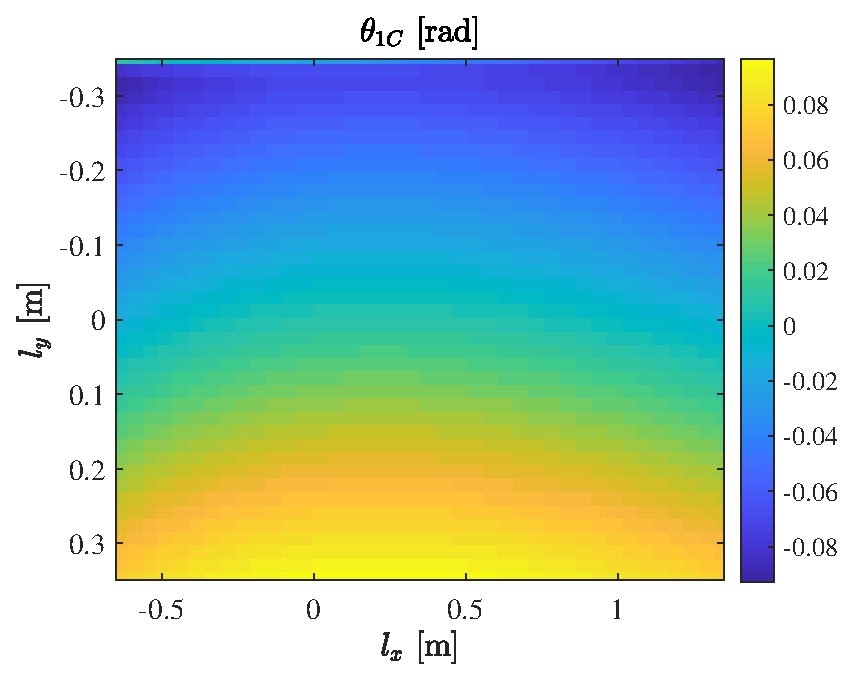
\includegraphics[width=60mm]{graficos/theta1CVH2lxy10ms}}
	\subfigure[Ángulo de paso cíclico longitudinal en función de la posición relativa a $O_f$ de la carga 2 para una velocidad de vuelo de 50 m/s.]{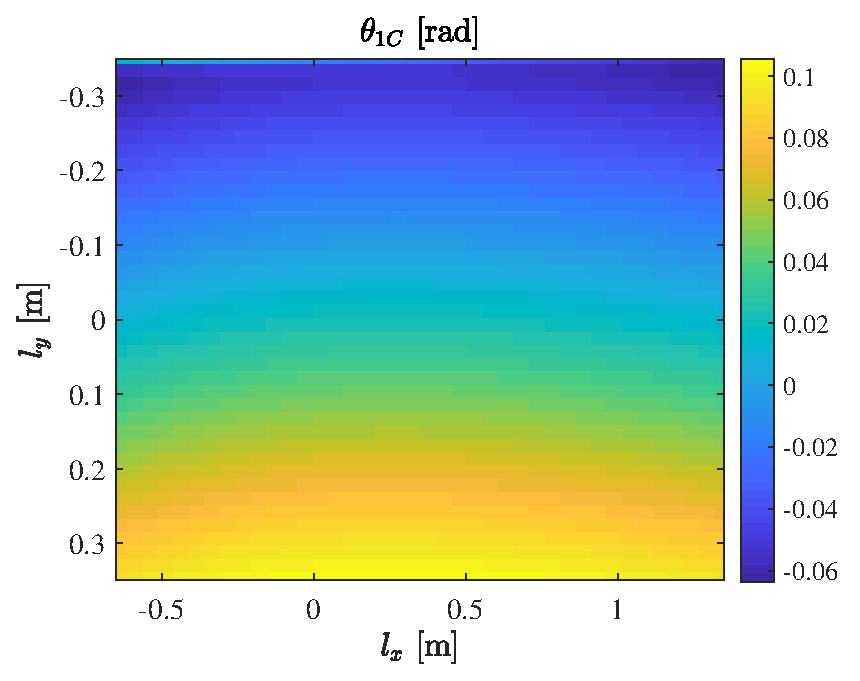
\includegraphics[width=60mm]{graficos/theta1CVH2lxy50ms}}
	\caption{Ángulo de paso cíclico longitudinal en función de la posición relativa a $O_f$ de la carga 2.}
	\label{theta1CVH2lxy}
\end{figure}
\begin{figure}
	\centering
	\subfigure[Ángulo de paso cíclico longitudinal en función de la posición relativa a $O_f$ de la carga 3 para una velocidad de vuelo de 10 m/s.]{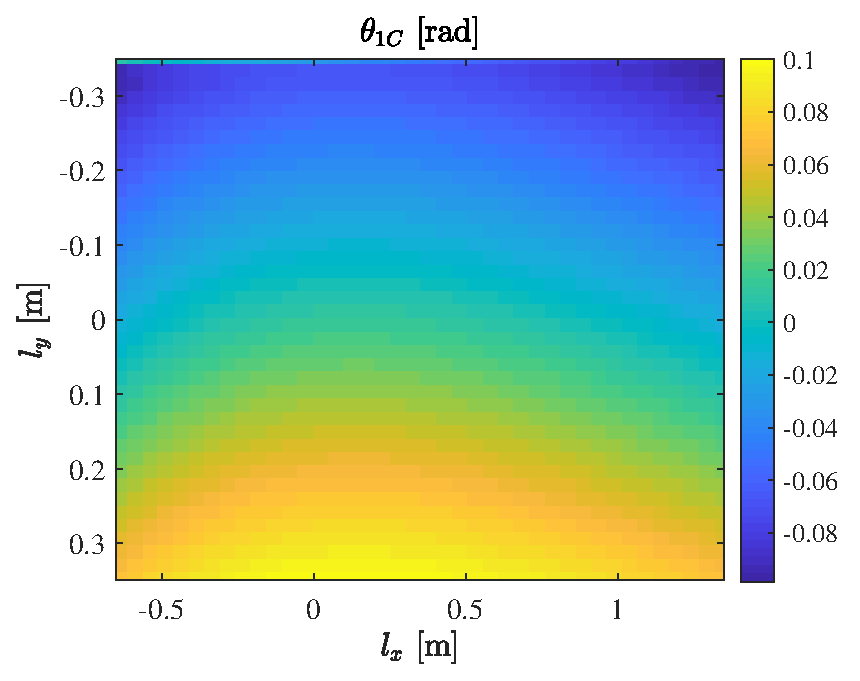
\includegraphics[width=60mm]{graficos/theta1CVH3lxy10ms}}
	\subfigure[Ángulo de paso cíclico longitudinal en función de la posición relativa a $O_f$ de la carga 3 para una velocidad de vuelo de 50 m/s.]{\includegraphics[width=60mm]{graficos/theta1CVH3lxy50ms}}
	\caption{Ángulo de paso cíclico longitudinal en función de la posición relativa a $O_f$ de la carga 3.}
	\label{theta1CVH3lxy}
\end{figure}

La variación de los ángulos de paso cíclico con la posición de la carga son más acusados, pero la velocidad de vuelo apenas influye en la misma. Para el paso cíclico longitudinal los máximos valores se dan para cargas centradas longitudinalmente y situadas a la izquierda del fuselaje, independientemente de la velocidad, aunque estos valores crecen ligeramente con esta como se puede observa en las gráficas \ref{theta1CVH2lxy} y \ref{theta1CVH3lxy}.

\begin{figure}
	\centering
	\subfigure[Ángulo de paso cíclico lateral en función de la posición relativa a $O_f$ de la carga 2 para una velocidad de vuelo de 10 m/s.]{\includegraphics[width=60mm]{graficos/theta1SVH2lxy10ms}}
	\subfigure[Ángulo de paso cíclico lateral en función de la posición relativa a $O_f$ de la carga 2 para una velocidad de vuelo de 50 m/s.]{\includegraphics[width=60mm]{graficos/theta1SVH2lxy50ms}}
	\caption{Ángulo de paso cíclico lateral en función de la posición relativa a $O_f$ de la carga 2.}
	\label{theta1SVH2lxy}
\end{figure}
\begin{figure}
	\centering
	\subfigure[Ángulo de paso cíclico lateral en función de la posición relativa a $O_f$ de la carga 3 para una velocidad de vuelo de 10 m/s.]{\includegraphics[width=60mm]{graficos/theta1SVH3lxy10ms}}
	\subfigure[Ángulo de paso cíclico lateral en función de la posición relativa a $O_f$ de la carga 3 para una velocidad de vuelo de 50 m/s.]{\includegraphics[width=60mm]{graficos/theta1SVH3lxy50ms}}
	\caption{Ángulo de paso cíclico lateral en función de la posición relativa a $O_f$ de la carga 3.}
	\label{theta1SVH3lxy}
\end{figure}

En cambio, la variación de los ángulos de paso cíclico lateral se da de forma totalmente opuesta, alcanzándose los mínimos para cargas centradas longitudinalmente y situadas a la izquierda del fuselaje, y de nuevo esta distribución se repite tanto a altas como bajas velocidades.

Las mayores variaciones observadas para el efecto de la carga se encuentran para el valor del paso cíclico lateral a altas velocidades, los cuales alcanzan valores de hasta 0.02 rad superiores para la carga 3, de mayor tamaño y masa.

\begin{figure}
	\centering
	\subfigure[Ángulo de cabeceo de la aeronave en función de la posición relativa a $O_f$ de la carga 2 para una velocidad de vuelo de 10 m/s.]{\includegraphics[width=60mm]{graficos/CabVH2lxy10ms}}
	\subfigure[Ángulo de cabeceo de la aeronave en función de la posición relativa a $O_f$ de la carga 2 para una velocidad de vuelo de 50 m/s.]{\includegraphics[width=60mm]{graficos/CabVH2lxy50ms}}
	\caption{Ángulo de cabeceo de la aeronave en función de la posición relativa a $O_f$ de la carga 2.}
	\label{CabVH2lxy}
\end{figure}
\begin{figure}
	\centering
	\subfigure[Ángulo de cabeceo de la aeronave en función de la posición relativa a $O_f$ de la carga 3 para una velocidad de vuelo de 10 m/s.]{\includegraphics[width=60mm]{graficos/CabVH3lxy10ms}}
	\subfigure[Ángulo de cabeceo de la aeronave en función de la posición relativa a $O_f$ de la carga 3 para una velocidad de vuelo de 50 m/s.]{\includegraphics[width=60mm]{graficos/CabVH3lxy50ms}}
	\caption{Ángulo de cabeceo de la aeronave en función de la posición relativa a $O_f$ de la carga 3.}
	\label{CabVH3lxy}
\end{figure}

\begin{figure}
	\centering
	\subfigure[Ángulo de balanceo de la aeronave en función de la posición relativa a $O_f$ de la carga 2 para una velocidad de vuelo de 10 m/s.]{\includegraphics[width=60mm]{graficos/BalanVH2lxy10ms}}
	\subfigure[Ángulo de balanceo de la aeronave en función de la posición relativa a $O_f$ de la carga 2 para una velocidad de vuelo de 50 m/s.]{\includegraphics[width=60mm]{graficos/BalanVH2lxy50ms}}
	\caption{Ángulo de balanceo de la aeronave en función de la posición relativa a $O_f$ de la carga 2.}
	\label{BalanVH2lxy}
\end{figure}
\begin{figure}
	\centering
	\subfigure[Ángulo de balanceo de la aeronave en función de la posición relativa a $O_f$ de la carga 3 para una velocidad de vuelo de 10 m/s.]{\includegraphics[width=60mm]{graficos/BalanVH3lxy10ms}}
	\subfigure[Ángulo de balanceo de la aeronave en función de la posición relativa a $O_f$ de la carga 3 para una velocidad de vuelo de 50 m/s.]{\includegraphics[width=60mm]{graficos/BalanVH3lxy50ms}}
	\caption{Ángulo de balanceo de la aeronave en función de la posición relativa a $O_f$ de la carga 3.}
	\label{BalanVH3lxy}
\end{figure}

En lo que respecta a los ángulos de Euler, la evolución resulta curiosa aunque no sorprendente; en las gráficas \ref{CabVH2lxy} y \ref{CabVH3lxy} se observa que el valor del ángulo de cabeceo de la aeronave no depende de la posición lateral de la carga, al igual que en las gráficas \ref{BalanVH2lxy} y \ref{BalanVH3lxy} el ángulo de balanceo no varía con la posición longitudinal de las mismas.

En el caso del cabeceo, los máximos valores se alcanzan para cargas centradas, siendo ligeramente mayor el incremento para altas velocidades. Las diferencias entre las cargas también son claras, a mayor carga, mayores son las diferencias entre los valores máximo y mínimo existentes. Para el balanceo, los máximos aparecen para cargas en la parte derecha del vehículo, no influyendo tanto en este caso la velocidad de vuelo o la carga embarcada.

\begin{figure}
	\centering
	\subfigure[Ángulo de paso colectivo del rotor antipar en función de la posición relativa a $O_f$ de la carga 2 para una velocidad de vuelo de 10 m/s.]{\includegraphics[width=60mm]{graficos/theta0raVH2lxy10ms}}
	\subfigure[Ángulo de paso colectivo del rotor antipar en función de la posición relativa a $O_f$ de la carga 2 para una velocidad de vuelo de 50 m/s.]{\includegraphics[width=60mm]{graficos/theta0raVH2lxy50ms}}
	\caption{Ángulo de paso colectivo del rotor antipar en función de la posición relativa a $O_f$ de la carga 2.}
	\label{theta0raVH2lxy}
\end{figure}
\begin{figure}
	\centering
	\subfigure[Ángulo de paso colectivo del rotor antipar en función de la posición relativa a $O_f$ de la carga 3 para una velocidad de vuelo de 10 m/s.]{\includegraphics[width=60mm]{graficos/theta0raVH3lxy10ms}}
	\subfigure[Ángulo de paso colectivo del rotor antipar en función de la posición relativa a $O_f$ de la carga 3 para una velocidad de vuelo de 50 m/s.]{\includegraphics[width=60mm]{graficos/theta0raVH3lxy50ms}}
	\caption{Ángulo de paso colectivo del rotor antipar en función de la posición relativa a $O_f$ de la carga 3.}
	\label{theta0raVH3lxy}
\end{figure}

Por último, el ángulo de paso colectivo del rotor antipar (gráficas \ref{theta0raVH2lxy} y \ref{theta0raVH3lxy}) sigue una evolución similar al del rotor principal, siendo los máximos a velocidades bajas para cargas centradas longitudinalmente y en la parte izquierda del fuselaje, invirtiéndose el efecto de la posición longitudinal para velocidades. El incremento de carga en este caso acusa más las diferencias entre los valores máximos y mínimos del paso, pero sus valores absolutos apenas varían 0.005 rad.
